%&../settings/preamble.main

\ifsubfile
\usepackage[newfloat, cachedir=_minted-cache, outputdir=../build]{minted}
\usepackage{../libraries/set-minted}

\pagestyle{plain}
\setcounter{chapter}{12}

% arara: pdflatex: { options: ["--output-directory=../build/chapters"], shell: yes, draft: yes, synctex: no }
% arara: pdflatex: { options: ["--output-directory=../build/chapters"], shell: yes, synctex: no }
\begin{document}
\fi
\chapter{Programmazione Dinamica}
\begin{fquote}[George Santayana][1905]
Those who cannot remember the past are condemned to repeat it
\end{fquote}

\section*{Introduzione}

La programmazione dinamica è un metodo per spezzare ricorsivamente un problema in
sottoproblemi, i quali vengono risolti una sola volta e la loro soluzione viene memorizzata in una tabella.
Nel caso il sottoproblema debba essere risolto nuovamente, si recupera la soluzione dalla tabella.
La tabella è facilmente indirizzabile: la sua consultazione costa \(\Omicron(1)\).

\begin{figure}[H]\centering
    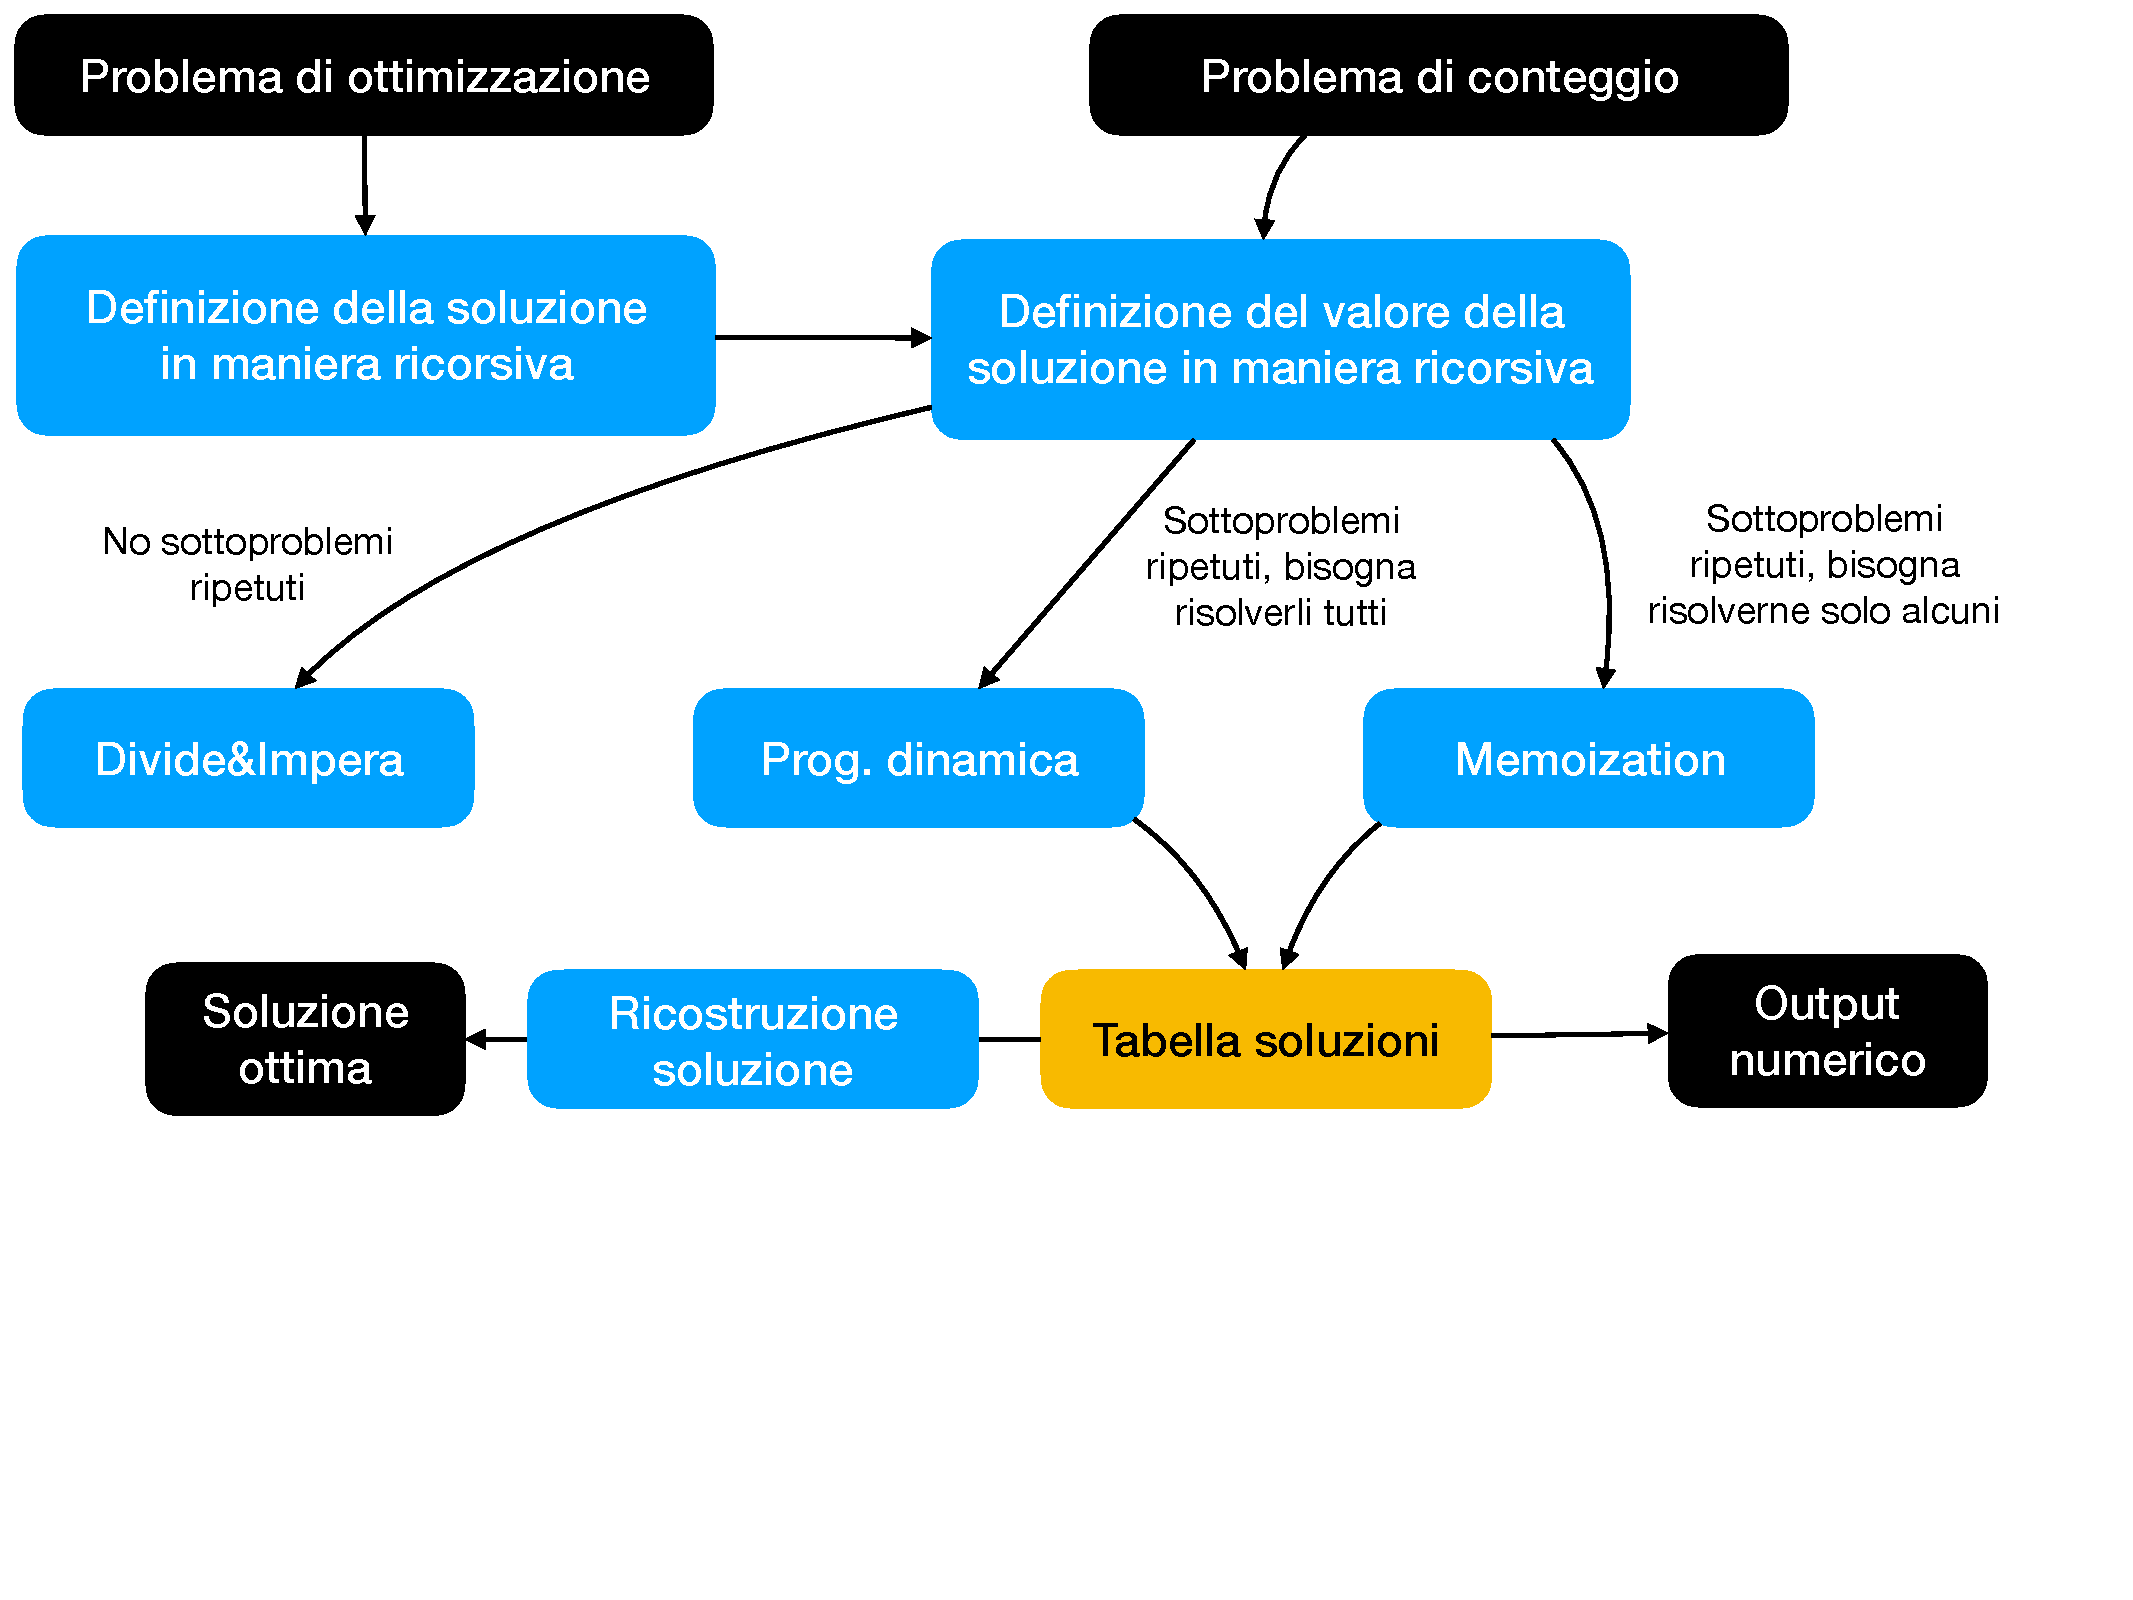
\includegraphics[width=.65\textwidth]{progrdyn}
    \caption{Approccio generale ad un problema}
\end{figure}

\subsection*{La programmazione dinamica nella storia}

Il termine \foreign{Dynamic Programming} è stato coniato da Richard Bellman agli inizi degli anni '50, nell'ambito dell'ottimizzazione matematica.
Inizialmente, si riferiva al processo di risolvere un problema compiendo le migliori decisioni una dopo l'altra.
\enquote{\foreign{Dynamic}} doveva dare un senso \enquote{temporale}, mentre \enquote{\foreign{Programming}} si riferiva all'idea di creare \enquote{programmazioni ottime}, per esempio nella logistica.
\`{E} possibile approfondire all'indirizzo \url{https://en.wikipedia.org/wiki/Dynamic_programming#History}.

La \emph{programmazione dinamica} è caratterizzata da 4 fasi principali:
\begin{enumerate}
    \item caratterizzare \emph{matematicamente} la struttura di una soluzione ottima;
    \item definire ricorsivamente il valore di una soluzione ottima;
    \item calcolare il valore di una soluzione ottima con approccio \foreign{bottom-up} ed utilizzare una tabella per memorizzare la soluzione dei sottoproblemi  ed utilizzarla per evitare di ripetere i calcoli più volte;
    \item ricostruire la soluzione ottima.
\end{enumerate}

\clearpage
\section{Domino}

\paragraph{Definizione del problema}
Il gioco del domino è basato su tessere di dimensione \(2 \times 1\).
Scrivere un algoritmo efficiente che prenda in input un intero \(n\) e restituisca il numero di possibili disposizioni di \(n\) tessere in un rettangolo \(2 \times n\).

\begin{figure}[H]\centering
    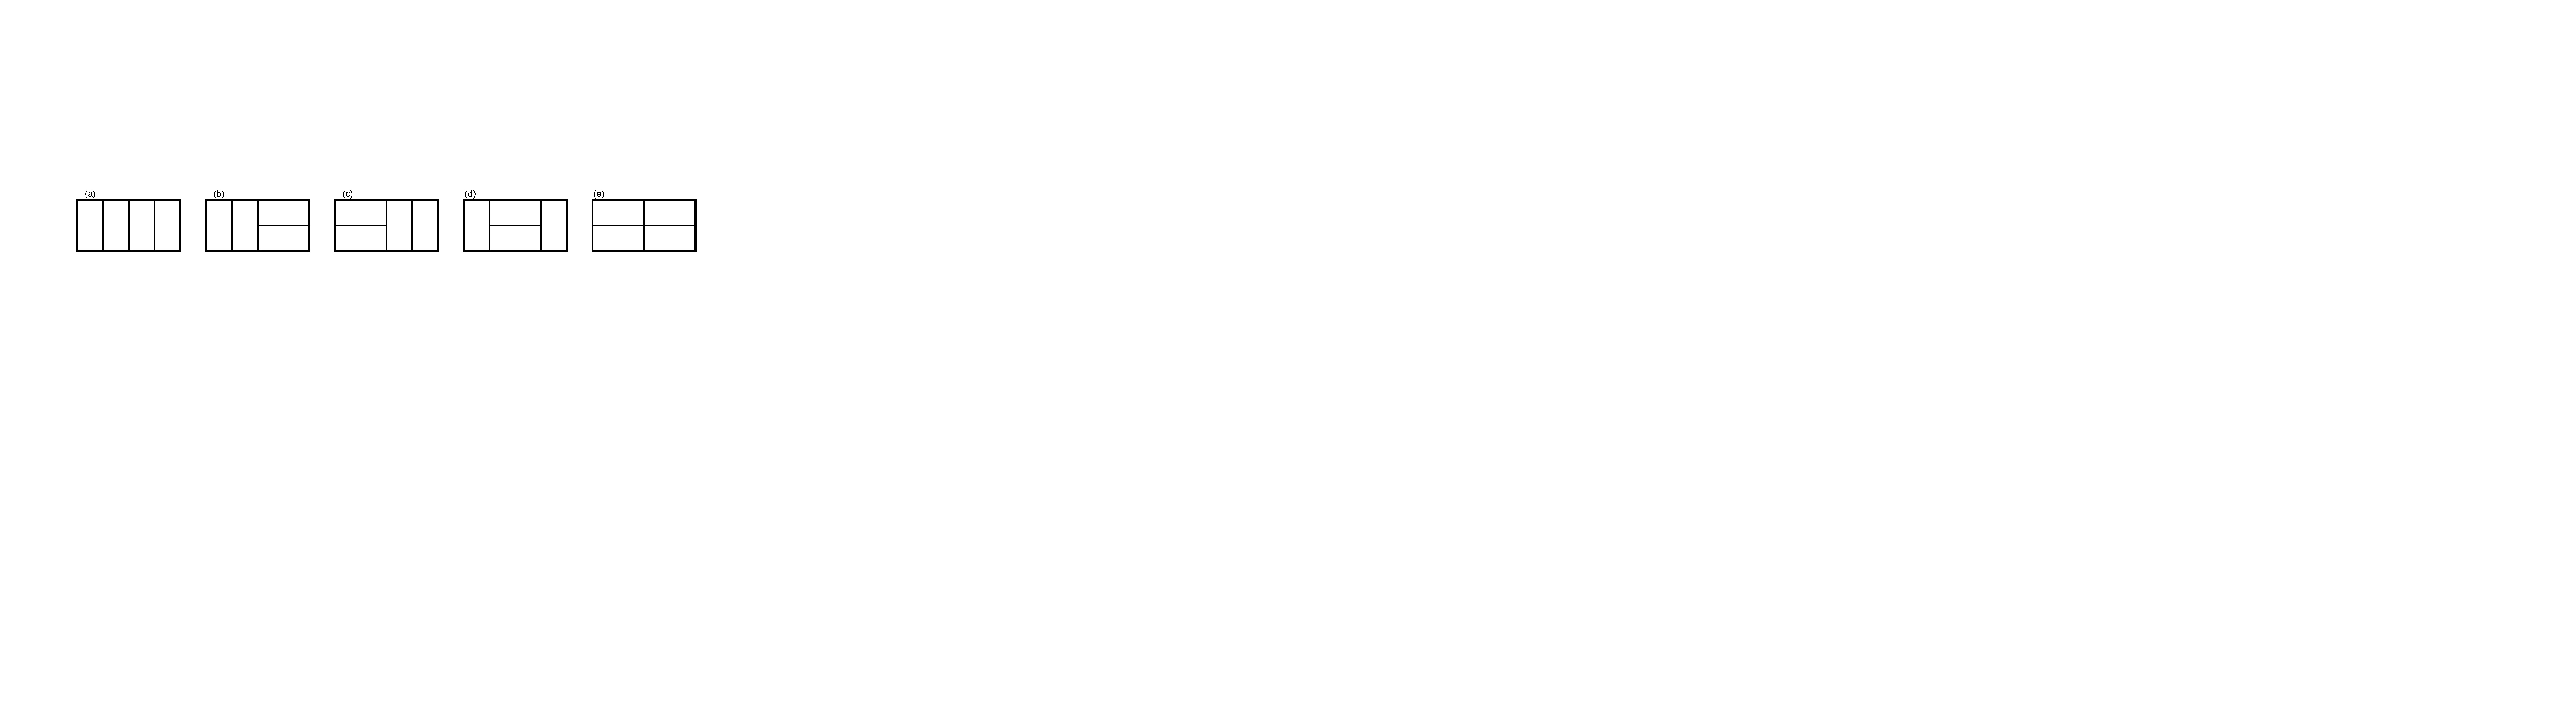
\includegraphics[width=1\textwidth]{domino}
    \caption[]{Rappresentazione delle cinque disposizioni possibili con cui è possibile riempire un rettangolo \(2 \times 4\).}
\end{figure}

\subsubsection{Definizione ricorsiva}

Definiamo una formula ricorsiva \(DP[n]\) che ci permetta di calcolare il numero di disposizioni possibili quando si hanno \(n\) tessere.
Con nessuna tessera (\(n=0\)) esiste una sola disposizione possibile.
Avendo a disposizione una tessera (\(n=1\)) è possibile disporla solo verticalmente.

Se posiziono una tessera in verticale, risolverò il problema di dimensione \(n-1\), mentre se la posiziono in orizzontale ne devo mettere due, risolvendo così il problema di dimensione \(n-2\).
Queste ultime due possibilità si sommano insieme (conteggio).
\[
    DP(n) =
    \begin{dcases}
    1                 & n \leqslant 1 \\
    DP[n-2] + DP[n-1] & n > 1 \\
    \end{dcases}
\]

La serie generata è una successione di Fibonacci.
\(DP[n]\) infatti è pari al \(n + 1\)-esimo numero della serie.

\subsubsection{Algoritmo ricorsivo}

L'algoritmo che viene scaturito dalla definizione ricorsiva del problema è il seguente:

\begin{algorithm}[H]
    \caption{Algoritmo \emph{ricorsivo} che risolve il problema Domino}
    %&../preamble

% arara: pdflatex: { synctex: no }
% arara: latexmk: { clean: partial }
\ifstandalone
\begin{document}
\begin{algorithm}[H]
\fi

\prototype{\Int \fibonacciRic{\Int n}}{
	\eIf{\( n \leqslant 1 \)}{
		\Return \(1\)\;
	}{
		% \tcp{due chiamate ricorsive \(time \to \Omicron(2^n)\)}
		\Return \(\fibonacciRic{\(n-1\)} + \fibonacciRic{\(n-2\)}\)\;
	}
}

\ifstandalone
\end{algorithm}
\end{document}
\fi

\end{algorithm}

\paragraph{Analisi della complessità}
L'equazione di ricorrenza associata a \fibonacciRic è la seguente:
\[
    T(n) =
    \begin{dcases}
    1                   & n \leqslant 1 \\
    T(n-1) + T(n-2) + 1 & n > 1 \\
    \end{dcases}
\]
\`{E} una ricorrenza lineare di ordine costante, per calcolare la sua complessità applichiamo quindi il \foreign{master theorem}: i fattori moltiplicativi di \(T(n-1)\) e \(T(n-2)\) sono \(a_1 = 1\) e \(a_2 = 1\) rispettivamente, possiamo raccogliergli in \(a = a_1 + a_2 = 2\), il fattore \(\beta\) risulta pari a \(0\), in quanto \(n^0=1\).
Possiamo quindi concludere che la complessità dell'algoritmo è \(\Theta(a^n \cdot n^\beta) = \Theta(2^n)\).

L'albero di ricorsione generato dall'algoritmo è il seguente:

\begin{figure}[H]\centering
    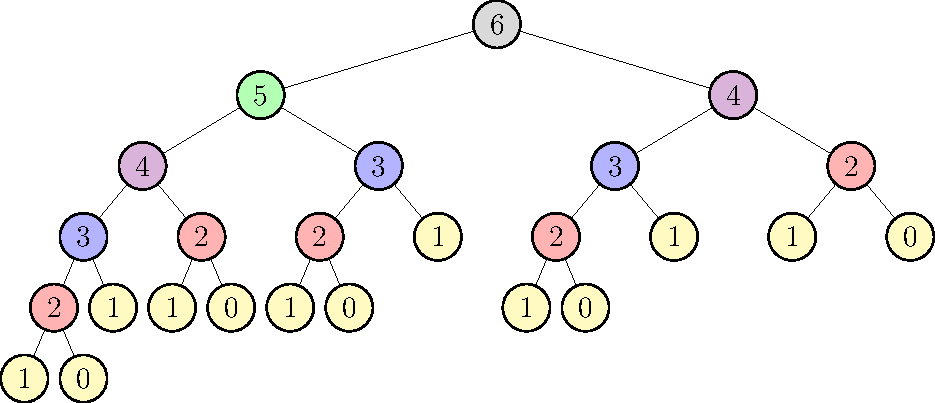
\includegraphics[width=.7\textwidth]{fibonacci-tree}
    \caption[]{Albero di ricorsione per \fibonacciRic. Possiamo notare che molti sottoproblemi vengono ripetuti.}
\end{figure}

\subsubsection{Come evitare di risolvere un problema più di una volta}

Dall'albero di ricorsione possiamo notare che molti sottoproblemi vengono ripetuti.
Per evitare che questo avvenga memorizziamo il risultato ottenuto risolvendo un particolare
problema in una \textbf{tabella DP}, la quale sarà un vettore, una matrice o dizionario dipendentemente dalle nostre esigenze.
La tabella conterrà un elemento per ogni sottoproblema che dobbiamo risolvere.
Memorizzeremo i casi base nelle relative posizioni.
Dopodiché l'iterazione sarà \foreign{bottom-up}: partiremo dai casi base e andremo verso problemi via via sempre più grandi fino a risolvere il problema originale.

\begin{algorithm}[H]
    \caption{Algoritmo \emph{iterativo} che risolve il problema Domino}
    %&../preamble

% arara: pdflatex: { synctex: no }
% arara: latexmk: { clean: partial }
\ifstandalone
\begin{document}
\begin{algorithm}[H]
\fi

\prototype{\Int \fibonacciIter{\Int \(n\)}}{

	\BlankLine
	\(DP\) \Assign \new \Array{\Int}[0][n] \tcp{inizializzo la \enquote{tabella} DP}
	\(DP[0] \Assign DP[1] \Assign 1\) \tcp{inserisco i casi base}

	\BlankLine
	\tcp{computo i valori successivi sulla base dei valori precedenti}
	\From{\(i \Assign 2\) \DownTo \(n\)}{
		\(DP[i]\) \Assign \(DP[i-1] + DP[i-2]\)\;
	}

	\BlankLine
	\Return \(DP[n]\) \tcp{restituisco il valore \(n\)-esimo richiesto}
}

\ifstandalone
\end{algorithm}
\end{document}
\fi

\end{algorithm}
\paragraph{Analisi della complessità}
% La complessità in tempo è lineare, come lo è la complessità spaziale.
La complessità in tempo è \(T(n) = \Theta(n)\), quella in spazio è \(S(n) = \Theta(n)\).
\`{E} possibile migliorare l'algoritmo riducendo lo spazio utilizzato.

\begin{table}[H]\centering
    \caption{I casi base vengono inseriti manualemente nelle relative posizioni.\\Ogni valore \(i\)-esimo successivo viene computato sulla base dei suoi valori precedenti \(i-1\) e \(1-2\).}
    % 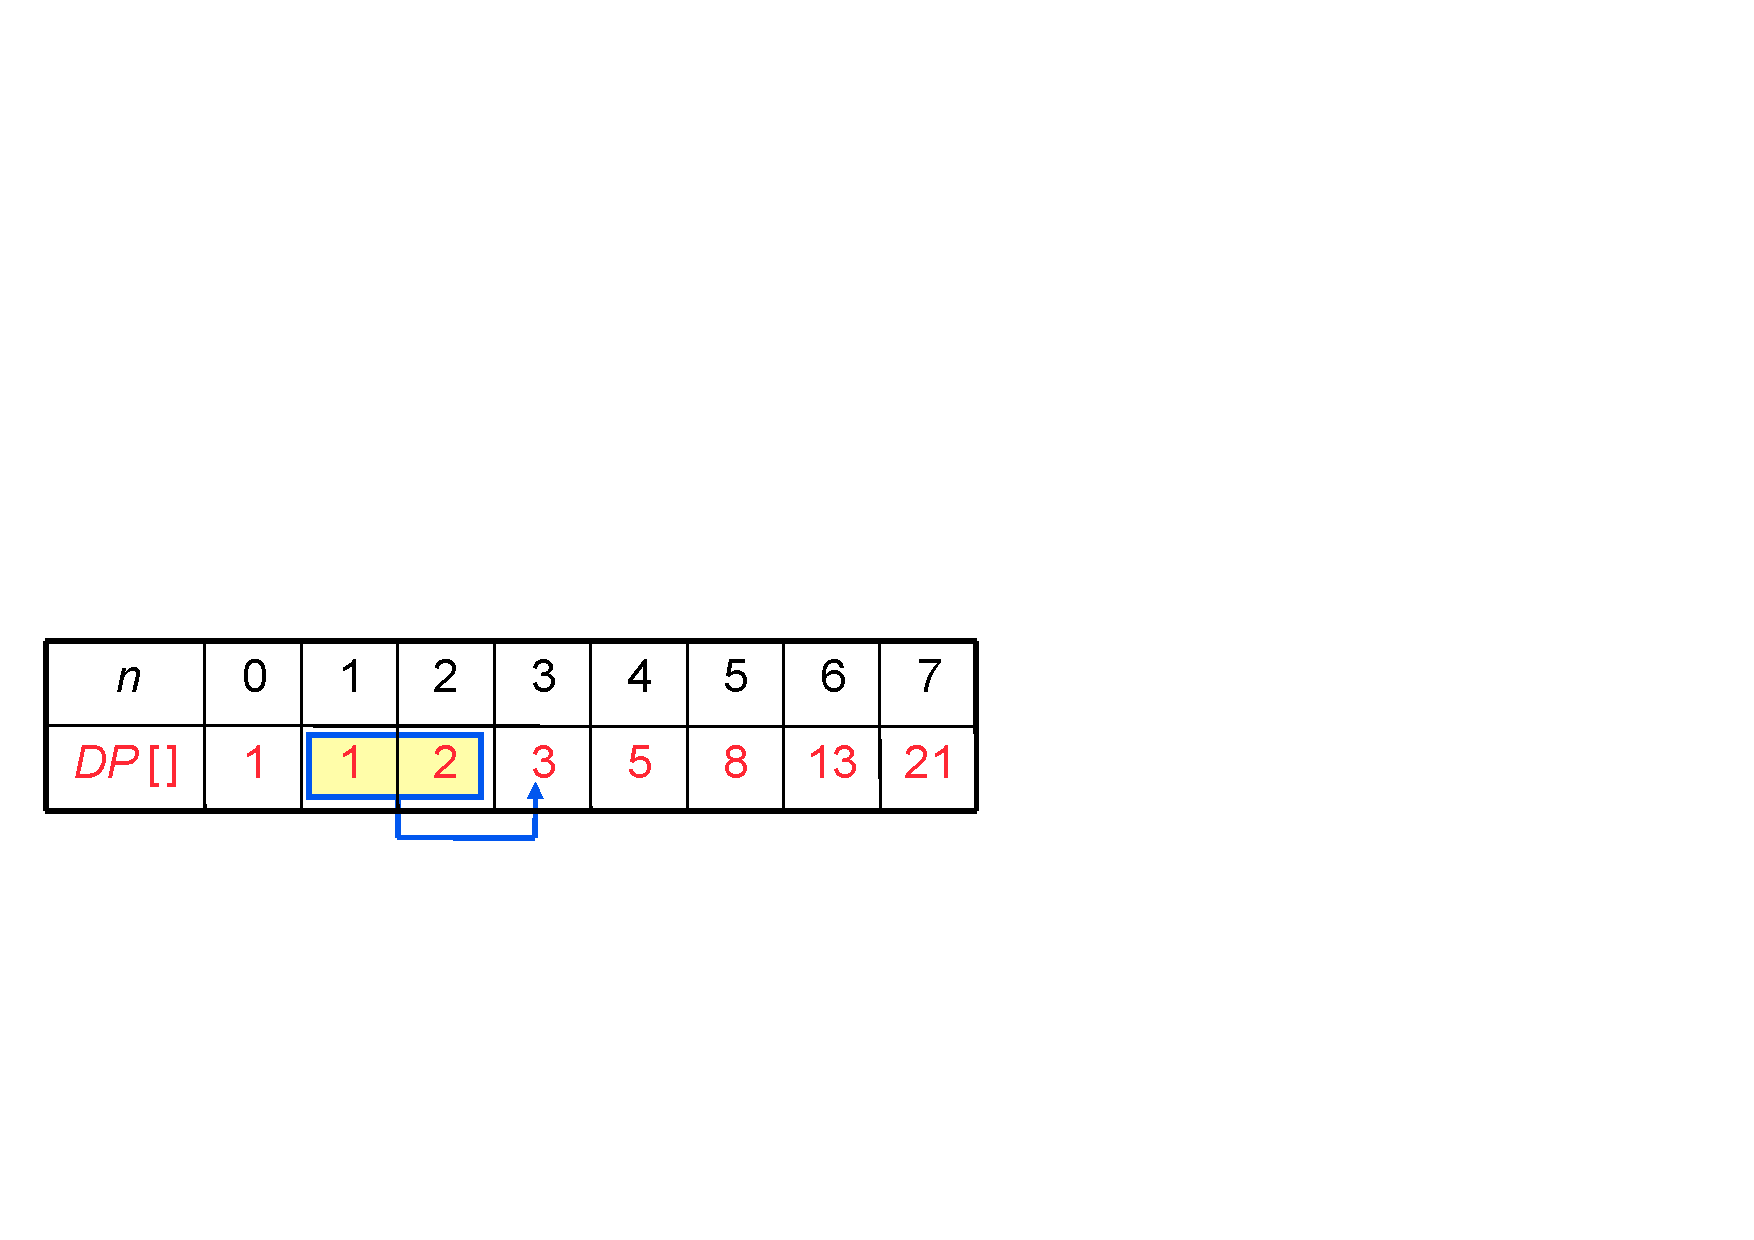
\includegraphics[width=.4\textwidth]{fib-table1}
    \begin{tabular}{@{} *{9}{C} @{}}
    \toprule
        n & 0 & 1 & 2 & 3 & 4 & 5 & 6 & 7 \\
    \midrule
        DP[n] & \emph{1} & \emph{1} & 2 & 3 & 5 & 8 & 13 & 21 \\
    \bottomrule
    \end{tabular}
\end{table}

\begin{algorithm}[H]
    \caption{Algoritmo \emph{iterativo che ottimizza lo spazio utilizzato} che risolve il problema Domino}
    %&../preamble

% arara: pdflatex: { synctex: no }
% arara: latexmk: { clean: partial }
\ifstandalone
\begin{document}
\begin{algorithm}[H]
\fi

\prototype{\Int \fibonacci{\Int \(n\)}}{

	\BlankLine
	\Int \(DP_0 \Assign 1\)\;
	\Int \(DP_1 \Assign 1\)\;
	\Int \(DP_2 \Assign 1\)\;

	\BlankLine
	\From{\(i \Assign 2\) \DownTo \(n\)}{
		\(DP_0 \Assign DP_1\)\;
		\(DP_1 \Assign DP_2\)\;
		\(DP_2 \Assign DP_0 + DP_1\)\;
	}

	\BlankLine
	\Return \(DP_2\)\;
}

\ifstandalone
\end{algorithm}
\end{document}
\fi

\end{algorithm}
\paragraph{Analisi della complessità}
Questa implementazione ha costo costante nello spazio \(S(n) = \Theta(1)\).

\renewcommand\arraystretch{1.4}
\begin{table}[H]\centering
    % 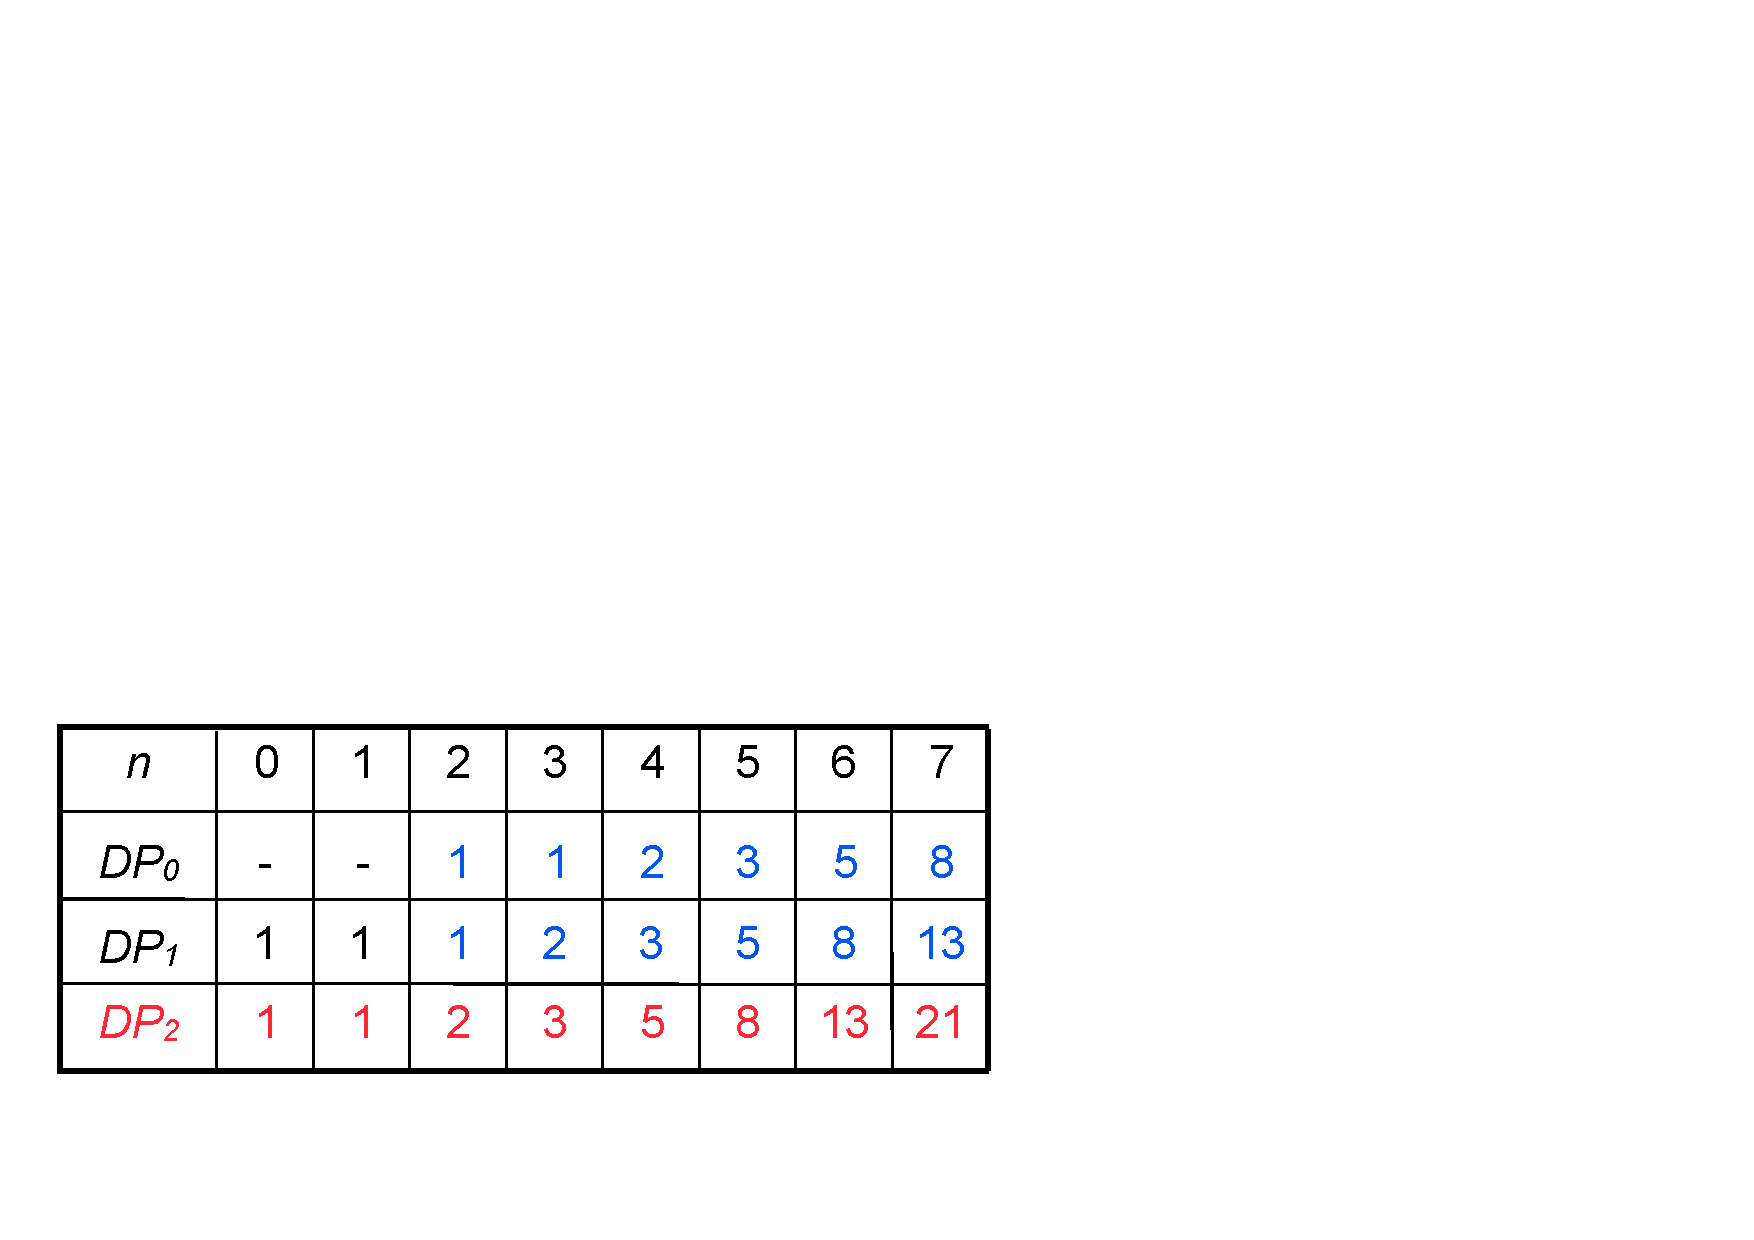
\includegraphics[width=.4\textwidth]{fib-table2}
    \begin{tabular}{@{} C ? *{7}{C|} C @{}}
        n & 0 & 1 & 2 & 3 & 4 & 5 & 6 & 7 \\
    \thickrule
        {DP[n]_0} & - & - & 1 & 1 & 2 & 3 & 5 & 8 \\
        {DP[n]_1} & \emph{1} & \emph{1} & 1 & 2 & 3 & 5 & 8 & 13 \\
        {DP[n]_2} & \emph{1} & \emph{1} & 2 & 3 & 5 & 8 & 13 & 21 \\
    \end{tabular}
\end{table}
\renewcommand\arraystretch{1}

Sotto il modello di costo logaritmico, le tre versioni hanno le complessità mostrate nella tabella.

\begin{table}[H]\centering
    \caption{Confronto delle varie versioni della funzione di fibonacci}
    \begin{tabular}{@{} ll cc @{}}
    \toprule
        Funzione & Tipologia & \(T(n)\) & \(S(n)\) \\
    \midrule
        \fibonacciRic &  ricorsiva & \(\Omicron(n2^n)\) & \(\Omicron(n^2)\) \\
    \lightrule
        \fibonacciIter &  iterativa & \(\Omicron(n^2)\) & \(\Omicron(n^2)\) \\
    \lightrule
        \fibonacci &  finale & \(\Omicron(n^2)\) & \(\Omicron(n)\) \\
    \bottomrule
    \end{tabular}
\end{table}

Si può fare meglio di così utilizzando l'esponenziazione di matrici basata su quadrati (per approfondimenti consultare \url{https://brilliant.org/wiki/fast-fibonacci-transform/}).

\clearpage
\section{Hateville}

\paragraph{Descrizione del problema}
Hateville è un villaggio particolare, composto da \(n\) case, numerate da \(1\) a \(n\) lungo una singola strada.
Ad Hateville ognuno odia i propri vicini della porta accanto, da entrambi i lati.
Quindi il vicino \(i\) odia i vicini \(i-1\) e \(i+1\) (se esistenti).
Hateville vuole organizzare una sagra e vi ha affidato il compito di raccogliere i fondi.
Ogni abitante \(i\) ha intenzione di donare una quantità \(D[i]\), ma non intende partecipare ad una raccolta fondi a cui partecipano uno o entrambi i propri vicini.

Dobbiamo scrivere un algoritmo che restituisca la quantità massima di fondi che può essere raccolta.

\paragraph{Consegne del problema}
I problemi che possono esserci posti sono due:
\begin{enumerate}
    \item scrivere un algoritmo che restituisca la quantità massima di fondi che può essere raccolta;
    \item scrivere un algoritmo che restituisca il sottoinsieme di indici \(S \subseteq \{1, \dots, n\}\) tale per cui la donazione totale \(T = \sum_{i \in S} D[i]\) è massimale.
\end{enumerate}
se risolviamo il primo siamo ad un passo dalla soluzione del secondo, mentre se risolviamo il primo abbiamo risolto necessariamente il primo.

\paragraph{Esempi di esecuzione}
Con un vettore di donazioni \(D = [4, 3, 6]\) la raccolta massima è \(10\), dato dall'insieme di indici \(\{1, 3\}\).
Mentre con un vettore di donazioni \(D = [10, 5, 5, 10]\) la raccolta massima è \(20\), dato dall'insieme di indici \(\{1, 4\}\).

La domanda che dobbiamo porci è la seguente: è possibile ridefinire una formula ricorsiva che ci permetta di calcolare il sottoinsieme di case che, se selezionate, dà origine alla maggior quantità di donazioni?

\subsection{Definizione ricorsiva}

Ridefiniamo il problema caratterizzandolo matematicamente.

Definiamo \(HV(i)\) uno dei possibili insiemi di indici da selezionare per ottenere una donazione ottimale delle prime \(i\) case di Hateville, numerate \(1, \dots, n\).
\(HV(n)\) diventa quindi la soluzione del problema originale.

\subsubsection{Passo ricorsivo}

Andiamo per passi.
Consideriamo il vicino \(i\)-esimo.
\begin{itemize}
    \item cosa succede se \textbf{non accetto} la sua donazione?
    Lo scarto.
    Proviamo ad esprimerlo in funzione dei problemi precedenti (dopotutto il problema viene risolto in maniera ricorsiva):
    \[HV(i) = HV(i-1)\]

    \item cosa succede se \textbf{accetto} la sua donazione?
    Accetto la donazione \(i\)-esima e scarto i vicini.
    In simboli:
    \[HV(i) = \{i\} \cup HV(i-2)\]

    \item a questo punto come faccio a \textbf{decidere} quale delle due opzioni scegliere?
    Semplicemente prendo quello che mi dà un guadagno maggiore.
    In simboli:
    \[HV(i) = highest(HV(i-1), \{i\} \cup HV(i-2))\]
\end{itemize}
La funzione \(highest\) restituisce l'insieme di valore massimo.

\subsection*{Sottostruttura ottima}

Quando voglio provare che una soluzione di programmazione dinamica è corretta devo riuscire a dimostrare che le mie possibili scelte sono quelle giuste.
Per dimostrarlo utilizziamo il teorema di sottostruttura ottima, che dice sostanzialmente che il modo in cui ho applicato la ricorsione è corretto.

Proviamo quindi a dimostrare le scelte fatte.
Il problema dato dalle prime \(i\) case è indicato con \(HV_{p}(i)\) e una (ce ne può essere più di una) soluzione ottima per questo problema è indicato con \(HV_{s}(i)\).

Se \(i \not\in HV_{s}i\) allora \(HV_{s}(i) = HV_{s}(i-1)\) (ossia se l'\(i\)-esimo elemento non appartiene alla soluzione del problema \(HV_{s}i\) allora abbiamo scartare quella donazione \(HV_{s}(i-1)\)), altrimenti se l'abbiamo accettata e quindi \(i \in HV_{s}i\) allora \(HV_{s}(i) = HV_{s}(i-2) \cup \{i\}\).

Se abbiamo la soluzione ottima, allora possiamo dimostrare che abbiamo la soluzione ottima per i rispettivi sottoproblemi (da qui sottostruttura).

\begin{note}
Nella maggior parte dei casi non è necessaria una dimostrazione della soluzione, ma basta un'intuizione.
\end{note}

\subsection{Dimostrazione sottostruttura ottima}

Ricordiamo che indichiamo con \(HV_{p}(i)\) il problema dato dalle prime \(i\) case e con \(HV_{s}(i)\) una delle possibili soluzioni ottime per questo problema.
Indichiamo inoltre con \(\abs{HV_{s}(i)}\) l'ammontare di donazioni per la soluzione ottima \(HV_{s}(i)\).

\begin{note}
Dobbiamo dimostrare separatamente il caso in cui prendiamo la donazione \(i\)-esima e il caso in cui non la prendiamo, in quanto sono eventi mutualmente esclusivi.
\end{note}

Entrambe le dimostrazioni procedono per assurdo.

\begin{proof}[Dimostrazione caso 1: \fbox{\(i \not\in HV_{s}(i)\)}]
Se non abbiamo preso la donazione \(i\)-esima vogliamo dimostrare che la soluzione ottima \(HV_{s}(i)\) è una soluzione ottima anche per il problema precedente \(HV_{p}(i-1)\).

Se così non fosse esisterebbe una soluzione (migliore) \(HV_{s}^{'} (i-1)\) per il problema \(HV_{p}(i-1)\) tale che l'ammontare delle donazioni del problema precedente sarebbe maggiore (in simboli \(\abs{HV_{s}^{'} (i-1)} > \abs{HV_{s}(i)}\)).
Ma allora \(HV_{s}^{'} (i-1)\) sarebbe una soluzione per \(HV_{p}(i)\)% (tale che \(\abs{HV_{s}^{'} (i-1)} > \abs{HV_{s}(i)}\))
, che è assurdo.
Quindi \(HV_{s}(i)\) è una soluzione ottima anche per \(HV_{p}(i-1)\).
\end{proof}

\begin{proof}[Dimostrazione caso 2: \fbox{\(i \in HV_{s}(i)\)}]
Se abbiamo preso l'\(i\)-esima donazione vogliamo dimostrare che \(i-1\) non appartiene alla soluzione ottima (in simboli \(i-1 \not\in HV_{s}(i)\)), altrimenti non sarebbe una soluzione ammissibile.
Quindi, se dalla soluzione ottima \(HV_{s}(i)\) togliessimo la donazione \(i\)-esima (\(HV_{s}(i) - \{i\}\)) questa dovrebbe essere una soluzione ottima per \(HV_{p} (i-2)\).

Se così non fosse, esisterebbe una soluzione \(HV_{s}^{'} (i-2)\) per il problema \(HV_{p} (i-2)\) tale che il suo guadagno sarebbe maggiore (in simboli \(\abs{HV_{s}^{'} (i-2)} > \abs{HV_{s} (i) - \{i\}}\)).
Ma allora \(HV_{s}^{'} (i-2) \cup \{i\}\) sarebbe una soluzione per \(HV_{p}(i)\)% (tale che \(\abs{HV_{s}^{'} (i-2) \cup \{i\}} > \abs{HV_{s} (i)}\))
, che è assurdo.
Quindi \(i-1 \not\in HV_s(i)\).
\end{proof}

\subsection{Completare la ricorsione}

Ragioniamo sui casi base.
Se ho \(0\) case il mio guadagno è zero: \(HV(0) = \emptyset\);
se ho una casa prendo semplicemente la sua donazione: \(HV(1) = \{1\}\).

Possiamo quindi scrivere la formula per calcolare la somma massima date \(i\) case:
\[
    HV(i) =
    \begin{dcases}
        0                                    & i = 0         \\
        \{1\}                                & i = 1         \\
        highest(HV(i-1), HV(i-2) \cup \{i\}) & i \geqslant 2 \\
    \end{dcases}
\]

Non vale la pena scrivere un algoritmo ricorsivo, basato su divide-et-impera, per risolvere il problema di Hateville poiché si risolverebbero molti sottoproblemi più volte.

\subsection{Memorizzare una tabella}

Facciamo qualche esempio di esecuzione.
Nel primo il vettore delle donazioni è \(D = [10, 5, 5, 8, 4, 7, 12]\), mentre nel secondo è \(D = [10, 1, 1, 10, 1, 1, 10]\).
Convincersi che gli insiemi risultanti sono corretti.

\begin{table}[H]\centering
    \begin{tabular}{@{} C *{8}{C} @{}}
    \toprule
        i & 0 & 1 & 2 & 3 & 4 & 5 & 6 & 7\\
    \midrule
        D & & 10 & 5 & 5 & 8 & 4 & 7 & 12\\
    \lightrule
        HV & \emptyset & \{1\} & \{1\} & \{1,3\} & \{1,4\} & \{1,3,5\} & \{1,4,6\} & \{1,3,5,7\}\\
    \bottomrule
    \end{tabular}
\end{table}

\begin{table}[H]\centering
    \begin{tabular}{@{} C *{8}{C} @{}}
    \toprule
        i & 0 & 1 & 2 & 3 & 4 & 5 & 6 & 7\\
    \midrule
        D &  & 10 & 1 & 1 & 10 & 1 & 1 & 10\\
    \lightrule
        HV & \emptyset & \{1\} & \{1\} & \{1,3\} & \{1,4\} & \{1,4\} & \{1,4,6\} & \{1,4,7\}\\
    \bottomrule
    \end{tabular}
\end{table}

A questo punto dobbiamo risolvere ancora due problemi:
\begin{enumerate}
    \item dobbiamo definire la funzione \(highest\) (ma è banale);
    \item dobbiamo memorizzare gli insiemi nella tabella.
\end{enumerate}
Memorizzare gli insiemi delle scelte nella tabella è costoso, quindi lo non faremo.
Costruiremo invece il valore della soluzione.
Così facendo eviteremo di memorizzare gli insiemi nella tabella e potremmo comunque ricostruire la soluzione a posteriori.

\subsubsection{Tabella di programmazione dinamica}

Indichiamo con \(DP[i]\) il \textbf{valore} della  massima quantità di donazioni che possiamo ottenere dalle prime \(i\) case di Hateville, e con \(DP[n]\) il valore della soluzione ottima.
%
Possiamo quindi riempire la tabella di programmazione dinamica nel seguente modo:
\[
    DP[i] =
    \begin{dcases}
        0                                  & i = 0 \\
        D[1]                               & i = 1 \\
    \maxFunction(DP[i-1], DP[i-2] + DP[i]) & i \geqslant 2 \\
    \end{dcases}
\]

Nel caso avessi \(0\) donatori allora la somma delle donazioni sarà \(0\).
Mentre nel caso abbia un solo donatore (\(i=1\)) allora prenderò la sua donazione (\(D[1]\)).
Infine nel caso avessi \(2\) o più donatori allora prendere una scelta: o scarterò quella donazione, quindi non considererò più quell'indice (\(DP[i-1]\)), o la accetter (\(+ DP[i]\)) e dovrò scartare a priori la scelta del suo vicino (\(DP[i-2]\)).
La sceltà è rappresentata dalla funzione \maxFunction che selezionerà quale fra le due scelte sarà quella più conveniente.

\begin{note}
Non memorizziamo più insiemi, ma valori.
Infatti non effettuiamo più l'unione di insiemi ma la somma fra i valori contenuti all'interno della tabella.
\end{note}

Dall'equazione di ricorrenza possiamo scrivere in modo naturale un algoritmo iterativo che risolve questo particolare problema.
Nel caso volessimo implementare un algoritmo ricorsivo allora dovremmo utilizzare la tecnica della \foreign{memoization} che vedremo più avanti.

\begin{algorithm}[H]
    \caption{Algoritmo iterativo che risolve il problema Hateville}
    %&../preamble

% arara: pdflatex: { synctex: no }
% arara: latexmk: { clean: partial }
\ifstandalone
\begin{document}
\begin{algorithm}[H]
\fi

\prototype{\Int \hateville{\Array{\Int} D, \Int n}}{

	\BlankLine
	\tcp{creo la tabella, un vettore in questo caso}
	\Array{\Int} \(DP\) \Assign \new \Array{\Int}[0][n]\;

	\BlankLine
	\tcp{inserisco i casi base}
	\(DP[0] \Assign 0\) \tcp{nessun donatore}
	\(DP[1] \Assign D[1]\) \tcp{un solo donatore}

	\BlankLine
	\tcp{calcolo il valore \(n\)-esimo}
	\From{\(i \Assign 2\) \DownTo \(n\)}{
		\(DP[i]\) \Assign \maxFunction{\(DP[i-1]\), \(DP[i-2] + D[i]\)}
	}

	\BlankLine
	\tcp{restituisco il valore \(n\)-esimo}
	\Return \(DP[n]\)\;
}

\ifstandalone
\end{algorithm}
\end{document}
\fi

\end{algorithm}

Stiamo calcolando la soluzione per ogni possibile sottoproblema (\(n+1\)) qual è il valore massimo della soluzione.
Questa soluzione ha complessità \(\Theta(n)\) in quanto dobbiamo fare \(\Theta(n)\) per ottenere il risultato.

\subsubsection{Soluzione con linguaggi di programmazione}

Vediamo un paio di implementazioni con \enquote{veri} linguaggi di programmazione.
Gli indici differiscono dalla notazione matematica.

\begin{code}
\begin{minted}{java}
public int hateville(int[] D, int n) {
    int[] DP = new int[n+1];
    DP[0] = 0;
    DP[1] = D[0]; // l'indice parte da \(0\)
    for (int i=2; i <= n; i++) {
        DP[i] = max(DP[i-1], DP[i-2] + D[i-1]); // devo prendere la donazione \(i-1\)
    }

    return DP[n];
}
\end{minted}
\captionof{listing}{Implementazione della soluzione in Java}
\end{code}

\begin{code}
\begin{minted}{python}
def hateville(D):
    DP = [ 0, D[0] ] # l'indice parte da \(0\)

    for i in range(1,len(D)): # scrittura più elegante
        DP.append( max(DP[-1], DP[-2] + D[i]) )

    return DP[-1]
\end{minted}
\captionof{listing}{Implementazione della soluzione in Python}
\end{code}

\subsection{Ricostruire la soluzione originale}

Questi sono i possibili risultati che possiamo ottenere applicando l'algoritmo.

\vspace{1ex}
\begin{minipage}{.5\linewidth}\centering
    \begin{tabular}{@{} >{$}c<{$} *{8}{c} @{}}
    \toprule
    i & 0 & 1 & 2 & 3 & 4 & 5 & 6 & 7\\
    \midrule
    D &  & 10 & 5 & 5 & 8 & 4 & 7 & 12\\
    \lightrule
    DP & 0 & 10 & 10 & 15 & 18 & 19 & 25 & 31\\
    \bottomrule
    \end{tabular}
\end{minipage}%
\begin{minipage}{.5\linewidth}\centering
    \begin{tabular}{@{} >{$}c<{$} *{8}{c} @{}}
    \toprule
    i & 0 & 1 & 2 & 3 & 4 & 5 & 6 & 7\\
    \midrule
    D &  & 10 & 1 & 1 & 10 & 1 & 1 & 10\\
    \lightrule
    DP & 0 & 10 & 10 & 11 & 20 & 20 & 21 & 30\\
    \bottomrule
    \end{tabular}
\end{minipage}
\vspace{1ex}

A questo punto abbiamo il valore della soluzione massimale, ma non abbiamo la soluzione, ossia l'insieme degli indici.

Per riscostruire la soluzione guardiamo l'elemento \(i\)-esimo presente nella tabella nella posizione \(DP[i]\), se la casa \(i\)-esima non è stata selezionata allora il valore di \(DP[i]\) deriva da \(DP[i-1]\), altrimenti (se la casa è stata selezionata) il suo valore deriva da \(DP[i-2] + D[i]\).
Se entrambe le equazioni sono vere, una vale l'altra.

Utilizziamo quindi questa informazione per ricostruire la soluzione in modo ricorsivo: per ricostruire la soluzione fino ad \(i\), calcoliamo i valori fino a \(i-2\) e aggiungiamo \(i\) (se la casa è stata selezionata), altrimenti li calcoliamo fino a \(i-1\) senza aggiungere nulla.

\begin{algorithm}[H]
    \caption{Ricostruire la soluzione generale di Hateville}
    %&../preamble

% arara: pdflatex: { synctex: no }
% arara: latexmk: { clean: partial }
\ifstandalone
\begin{document}
\begin{algorithm}[H]
\fi

\prototype{\Int \hateville{\Array{\Int} D, \Int n}}{

	\BlankLine
	\tcp{creo la tabella}
	\Array{\Int} \(DP\) \Assign \new \Array{\Int}[0][n]\;

	\BlankLine
	\tcp{inserisco i casi base}
	\(DP[0] \Assign 0\)\;
	\(DP[1] \Assign DP[1]\)\;

	\BlankLine
	\tcp{calcolo il valore \(i\)-esimo}
	\From{\(i \Assign 2\) \DownTo \(n\)}{
		\(DP[i]\) \Assign \maxFunction{\(DP[i-1]\), \(DP[i-2] + D[i]\)}
	}

	\BlankLine
	\tcp{restituisco il valore \(n\)-esimo}
	\Return \hatevilleSolution{\(DP\), \(D\), \(n\)}\;
}

\BlankLine
\tcp{ricostruisce l'insieme degli indici dato il valore massimale}
\prototype{\Int \hatevilleSolution{\Array{\Int} \(DP\), \Array{\Int} \(D\), \Int \(i\)}}{
	\params{i}[indice di scorrimento]

	\BlankLine
	\uIf(\tcp*[h]{nessun donatore}){\(i \Equal 0\)}{
		\Return \(\emptyset\)\;
	}
	\uElseIf(\tcp*[h]{un solo donatore}){\(i \Equal 1\)}{
		\Return \(\{1\}\)\;
	}
	\uElseIf(\Comment*[l]{se non c'è variazione fra valori consecutivi}){\(DP[i] \Equal DP[i-1]\)}{
		\Return \hatevilleSolution{\(DP\), \(D\), \(i-1\)} \tcp{scarto l'indice}
	}
	\Else(\tcp*[h]{c'è variazione fra valori consecutivi}){
		\Set \(sol =\) \hatevilleSolution{\(DP\), \(D\), \(i-2\)} \tcp{chiamo ricorsivamente l'algoritmo sull'indice \(i-2\)}
		\(sol\).\setInsert{i} \tcp{inserisco l'indice nell'insieme}

		\BlankLine
		\tcp{restituisco l'insieme degli indici}
		\Return \(sol\)\;
	}
}

\ifstandalone
\end{algorithm}
\end{document}
\fi

\end{algorithm}

Effettuo prima la chiamata ricorsiva e poi l'inserimento dell'indice all'interno dell'insieme così alla fine dell'esecuzione gli indici saranno nell'ordine corretto.

\paragraph{Analisi della complessità}
La complessità computazionale di \hatevilleSolution è \(T(n) = \Theta(n)\), quella spaziale è \(S(n) = \Theta(n)\).

\begin{note}
Non è possibile migliorare la complessità spaziale di \hateville poiché è necessario ricostruire la soluzione.
\end{note}

\clearpage
\section{Zaino}

\paragraph{Definizione informale del problema}
Dato un insieme di oggetti, ognuno caratterizzato da un \emph{peso} ed un \emph{profitto}, e uno \enquote{zaino} con un limite di capacità, individuare un sottoinsieme di oggetti il cui peso sia inferiore alla capacità dello zaino e in cui il valore totale degli oggetti sia massimale, ossia il più alto o uguale al valore di qualunque altro sottoinsieme di oggetti.

\paragraph{Definizione formale del problema}
Dati un vettore \(w\), dove \(w[i]\) è il \textbf{peso} (\foreign{weight}) dell'oggetto \(i\)-esimo, un vettore \(p\), dove \(p[i]\) è il \textbf{profitto} (\foreign{profit}) dell'oggetto \(i\)-esimo, e la \textbf{capacità} \(C\) dello zaino.
Bisogna trovare un insieme \(S \subseteq \{1, \dots, n\}\) tale che:
\begin{itemize}
    \item il \textbf{valore totale} deve essere minore o uguale alla capacità;
    \[w(S) = \sum_{i \in S} w[i] \leqslant C\]
    \item il \textbf{profitto totale} deve essere massimizzato.
    \[p(S) = \sum_{i \in S} p[i]\]
\end{itemize}

\paragraph{Esempi di esecuzione}
Con un vettore dei pesi \(w = [10, 4, 8]\) ed un vettore dei profitti \(p = [20, 6, 12]\) ed una capacità \(C=12\).
L'insieme degli indici da restituire è \(S = \{1\}\).
Mentre con un vettore dei pesi \(w = [10, 4, 8]\) ed un vettore dei profitti \(p = [20, 7, 15]\) ed una capacità sempre pari a \(C=12\).
L'insieme degli indici da restituire è \(S = \{2, 3\}\).

\subsubsection{Definizione matematica del valore della soluzione}

Dato uno zaino di capacità \(C\) e \(n\) oggetti caratterizzati da peso \(w\) e profitto \(p\), definiamo \(DP[i][c]\) come il massimo profitto che può essere ottenuto dai primi \(i \leqslant n\) oggetti contenuti in uno zaino di capacità \(c \leqslant C\).
Il massimo profitto ottenibile dal problema originale è rappresentato da \(DP[n][C]\).

\subsubsection{Passo ricorsivo}

Andiamo per passi.
Consideriamo l'oggetto \(i\)-esimo.
\begin{itemize}
    \item cosa succede se \textbf{non prendo} quell'oggetto?
    La capacità non cambia e non c'è profitto.
    Avanziamo con l'indice (\(i-1\)).
    \[DP[i][c] = DP[i-1][c]\]

    \item cosa succede se \textbf{prendo} quell'oggetto?
    Sottraiamo il peso dalla capacità (\(c - w[i]\)) e aggiungiamo il relativo profitto (\(+ p[i]\)).
    Avanziamo con l'indice (\(i-1\)).
    \[DP[i][c] = DP[i-1][c - w[i]] + p[i]\]

    \item a questo punto come faccio a \textbf{decidere} quale delle due opzioni scegliere?
    Semplicemente prendo quello che mi dà un guadagno maggiore.
    In simboli:
    \[DP[i][c] = \maxFunction(DP[i-1][c - w[i]] + p[i], DP[i-1][c])\]
\end{itemize}

\subsubsection{Completare la ricorsione}

Ragioniamo sui casi base.
Se non abbiamo più oggetti o se abbiamo finito la capacità dello zaino allora il nostro guadagno sarà \(0\).
E nel caso prendessimo un oggetto la nostra capacità diventasse negativa?
In quel caso mettiamo come valore convenzionale \(-\infty\).

Possiamo quindi scrivere la formula per calcolare il massimo guadagno dati \(i\) oggetti ed una capacità \(c\):
\[
    DP[i][c] =
    \begin{dcases}
        0                                                   & i=0\ \Or\ c=0     \\
        -\infty                                             & c<0               \\
        \maxFunction(DP[i-1][c - w[i]] + p[i], DP[i-1][c])) & \text{altrimenti} \\
    \end{dcases}
\]

\subsection{Algoritmo iterativo}

Dalla formula possiamo ricavare il seguente algoritmo iterativo.
\begin{algorithm}[H]
    \caption{Algoritmo \emph{iterativo} per la soluzione al problema dello zaino}
    %&../preamble

% arara: pdflatex: { synctex: no }
% arara: latexmk: { clean: partial }
\ifstandalone
\begin{document}
\begin{algorithm}[H]
\fi

\prototype{\Int \knapsack{\Array{\Int} \(w\), \Array{\Int} \(p\), \Int \(n\), \Int \(C\)}}{
    \params{w}[vettore dei pesi]
    \params{p}[vettore dei profitti]
    \params{n}[numero di oggetti]
    \params{C}[capacità massima dello zaino]

    \BlankLine
    \tcp{creo la tabella di programmazione dinamica}
    \(DP\) \Assign \new \Matrix{\Int}[0\dots n][0\dots C]\;

    \BlankLine
    \tcp{la inizializzo}
    \From{\(i \Assign 0\) \DownTo \(n\)}{
        \(DP[i][0] = 0\) \tcp{capacità nulla}
    }

    \BlankLine
    \From{\(c \Assign 0\) \DownTo \(C\)}{
        \(DP[0][c] = 0\) \tcp{nessun oggetto}
    }

    \BlankLine
    \tcp{calcolo caso per caso}
    \From{\(i \Assign 1\) \DownTo \(n\)}{

        \BlankLine
        \From{\(c \Assign 1\) \DownTo \(C\)}{

            \BlankLine
            \eIf(\tcp*[h]{se la capacità residua è sufficiente}){\(w[i] \leqslant c\)}{

                \BlankLine
                \(DP[i][c] = \maxFunction(DP[i-1][c - w[i]] + p[i], DP[i-1][c])\) \tcp{decido se prenderlo o scartarlo}
            }{
                \(DP[i][c] = DP[i-1][c]\) \tcp{lo scarto}
            }
        }
    }

    \BlankLine
    \tcp{restituisco il profitto massimo}
    \Return \(DP[n][C]\)\;
}

\ifstandalone
\end{algorithm}
\end{document}
\fi

\end{algorithm}

\paragraph{Esempio di esecuzione}
Con un vettore dei pesi \(w = [4, 2, 3, 4]\) e un vettore dei profitti \(p = [10, 7, 8, 6]\) ed una capacità di \(C=9\), la tabella di programmazione generata è la seguente:
\begin{table}[H]\centering
    \renewcommand*{\arraystretch}{1.4}
    \begin{tabular}{ c ? *{9}{C|} C }
        \diagbox[width=25pt, height=25pt]{i}{c} & \textbf{0} & \textbf{1} & \textbf{2} & \textbf{3} & \textbf{4} & \textbf{5} & \textbf{6} & \textbf{7} & \textbf{8} & \textbf{9}\\
    \thickrule
        \textbf{0} & \emph{0} & \emph{0} & \emph{0} & \emph{0} & \emph{0} & \emph{0} & \emph{0} & \emph{0} & \emph{0} & \emph{0} \\
    \hline
        \textbf{1} & \emph{0} & 0 & 0 & 0 & 10 & 10 & 10 & 10 & 10 & 10\\
    \hline
        \textbf{2} & \emph{0} & 0 & 7 & 7 & 10 & 10 & 17 & 17 & 17 & 17\\
    \hline
        \textbf{3} & \emph{0} & 0 & 7 & 8 & 10 & 15 & 17 & 18 & 18 & 25\\
    \hline
        \textbf{4} & \emph{0} & 0 & 7 & 8 & 10 & 15 & 17 & 18 & 18 & 25\\
    \end{tabular}
    \renewcommand*{\arraystretch}{1.0}
\end{table}

I valori in \textbf{grassetto} indicato numero di oggetti (\(i\)) e la capacità (\(c\)) dello zaino, mentre i valori in \emph{corsivo} sono i valori inizializzati della tabella.

La tabella viene riempita per righe.
Per capire come funziona l'algoritmo prendiamo in considerazione la seconda riga che corrisponde alla possibilità di prendere \(i=2\) oggetti: una volta raggiunta la capacità di \(c=2\) possiamo prendere l'oggetto con peso \(7\), una volta raggiunta la capacità di \(c=4\) devo scegliere il massimo profitto prendere l'oggetto \(10\) (\(DP[i-1][c - w[i]] + p[i]\)) e \(7\), ossia ignorarlo \(DP[i-1][c]\).
Quando raggiungo la capacità di \(c=6\) posso prendere entrambi gli oggetti per un profitto totale di \(17\).

\subsection{Algoritmo ricorsivo}

\paragraph{Complessità}
La complessità di \knapsack è \(\Theta(nC)\).
Osserviamo che \(C\) è parte dell'input (non è la dimensione del problema).
Applicchiamo quindi il criterio di costo logaritmico: per rappresentare \(C\) sono necessari \(k = \log_2 C\) bit, quindi la complessità è \(T(n) = \Omicron(n2^k)\). \knapsack è un algoritmo esponenziale.

\begin{algorithm}[H]
    \caption{Algoritmo \emph{ricorsivo} per la soluzione al problema dello zaino}
    %&../preamble

% arara: pdflatex: { synctex: no }
% arara: latexmk: { clean: partial }
\ifstandalone
\begin{document}
\begin{algorithm}[H]
\fi

\BlankLine
\tcp{metodo wrapper}
\prototype{\Int \knapsack{\Array{\Int} \(w\), \Array{\Int} \(p\), \Int \(n\), \Int \(C\)}}{

    \BlankLine
    \Return \knapsackRec{\(w\), \(p\), \(n\), \(C\)}\;
}

\BlankLine
\prototype{\Int \knapsackRec{\Array{\Int} \(w\), \Array{\Int} \(p\), \Int \(n\), \Int \(c\)}}{
    \params{c}[capacità residua]

    \BlankLine
    \uIf{\(c < 0\)}{
        \Return \(-\infty\)\;
        \BlankLine

    }
    \uElseIf{\(i \Equal 0\) \Or \(c \Equal 0\)}{
        \Return \(0\)\;
        \BlankLine

    }
    \Else{
        \Int \(nottaken\) \Assign \knapsackRec{\(w\), \(p\), \(i-1\), \(c\)}\;
        \Int \(taken\) \Assign \knapsackRec{\(w\), \(p\), \(i-1\), \(c-w[i]\)} \(+ p[i]\)\;

        \BlankLine
        \Return \maxFunction{\(nottaken\), \(taken\)}\;
    }
}

\ifstandalone
\end{algorithm}
\end{document}
\fi

\end{algorithm}

\paragraph{Analisi della complessità}
La funzione ricorsiva scaturita dalla funzione \knapsack è la seguente:
\[
    T(n) =
    \begin{dcases}
        1           & n \leqslant 1 \\
        2T(n-1) + 1 & n > 1         \\
    \end{dcases}
    = \Omicron(2^n)
\]
Non si può fare meglio di così.

\subsection{Memoization}

\begin{note}
Non tutti gli elementi della matrice sono necessari alla risoluzione del nostro problema.
\end{note}

Prendiamo l'esempio precedente.

\NewDocumentCommand{\red}{m}{\textcolor{red}{\textbf{#1}}}
\NewDocumentCommand{\green}{m}{\textcolor{ForestGreen}{\textbf{#1}}}

\begin{table}[H]\centering
    \renewcommand*{\arraystretch}{1.4}
    \begin{tabular}{ c ? *{9}{C|} C }
        \diagbox[width=25pt, height=25pt]{i}{c} & \textbf{0} & \textbf{1} & \textbf{2} & \textbf{3} & \textbf{4} & \textbf{5} & \textbf{6} & \textbf{7} & \textbf{8} & \textbf{9}\\
    \thickrule
        \textbf{0} & \emph{\red{0}} & \emph{\red{0}} & \emph{\red{0}} & \emph{\red{0}} & \emph{\red{0}} & \emph{\red{0}} & \emph{\red{0}} & \emph{\red{0}} & \emph{0} & \emph{\red{0}} \\
    \hline
        \textbf{1} & \emph{\red{0}} & 0 & \red{0} & \red{0} & \red{10} & \red{10} & \red{10} & \red{10} & 10 & \red{10}\\
    \hline
        \textbf{2} & \emph{0} & 0 & \red{7} & 7 & 10 & \red{10} & \red{17} & 17 & 17 & \red{17}\\
    \hline
        \textbf{3} & \emph{0} & 0 & 7 & 8 & 10 & \red{15} & 17 & 18 & 18 & \red{25}\\
    \hline
        \textbf{4} & \emph{0} & 0 & 7 & 8 & 10 & 15 & 17 & 18 & 18 & \red{25}\\
    \end{tabular}
    \renewcommand*{\arraystretch}{1.0}
\end{table}

I valori segnati in \red{rosso} sono gli unici necessari alla computazione della soluzione.

La \foreign{memoization} (annotazione) è una tecnica che fonde l'approccio di \emph{memorizzazione} della programmazione dinamica con l'approccio \foreign{top-down} di divide-et-impera.

Quando devo risolvere un sottoproblema prima controllo se l'ho già risolto, guardando nella cella corrispondente della tabella dove memorizzo i risultati, altrimenti lo calcolo al momento (\foreign{on-the-fly}) chiamando ricorsivamente i sottoproblemi e scrivendo i rispettivi risultati nella tabella.
In questo modo mi assicuro di fare il calcolo una volta sola ed evito di calcolare valori che non verranno mai usati.

Per indicare che il problema non è ancora stato risolto la inizializzo ad un valore speciale (\(-1\)).

\begin{algorithm}[H]
    \caption{Zaino con memoization}
    %&../preamble

% arara: pdflatex: { synctex: no }
% arara: latexmk: { clean: partial }
\ifstandalone
\begin{document}
\begin{algorithm}[H]
\fi

\BlankLine
\tcp{funzione wrapper}
\prototype{\Int \knapsack{\Array{\Int} \(w\), \Array{\Int} \(p\), \Int \(n\), \Int \(C\)}}{

    \BlankLine
    \(DP\) \Assign \new \Matrix{\Int}[1\dots n][1\dots C]\;

    \BlankLine
    \From{\(i \Assign 1\) \DownTo \(n\)}{

        \BlankLine
        \From{\(c \Assign 1\) \DownTo \(C\)}{

            \BlankLine
            \(DP[i][c] = -1\) \tcp{non ho ancora risolto questo sotto-problema}
        }
    }

    \BlankLine
    \Return \knapsackRec{\(w\), \(p\), \(n\), \(C\), \(DP\)}\;
}

\BlankLine
\prototype{\Int \knapsackRec{\Array{\Int} \(w\), \Array{\Int} \(p\), \Int \(n\), \Int \(c\), \Matrix{\Int}[][] \(DP\)}}{

    \BlankLine
    \uIf{\(c < 0\)}{
        \Return \(-\infty\)\;
        \BlankLine

    }
    \uElseIf{\(i \Equal 0\) \Or \(c \Equal 0\)}{
        \Return \(0\)\;
        \BlankLine

    }
    \Else{

        \BlankLine
        \If{\(DP[i][c] < 0\)}{

            \BlankLine
            \Int \(nottaken\) \Assign \knapsackRec{\(w\), \(p\), \(i-1\), \(c\), \(DP\)}\;
            \Int \(taken\) \Assign \knapsackRec{\(w\), \(p\), \(i-1\), \(c-w[i]\), \(DP\)} \(+ p[i]\)\;

            \BlankLine
            \(DP[i][c]\) \Assign \maxFunction{\(nottaken\), \(taken\)}\;
        }

        \BlankLine
        \Return \(DP[i][c]\)\;
    }
}

\ifstandalone
\end{algorithm}
\end{document}
\fi

\end{algorithm}
La tabella viene inizializzata esternamente, nella funzione \foreign{wrapper}, con un valore che non viene usato durante la procedura (\(-1\) nel caso vengano usati \emph{solo} valori positivi, \(-\infty\) nel caso vengano usati sia valori positivi che valori negativi).

\begin{minted}{python}
def knapsackRec(w, p, i, c, DP):
    if c < 0:
        return -math.inf
    elif i == 0 or c == 0:
        return 0
    else:
        if DP[i][c] < 0:
            nottaken = knapsackRec(w, p, i-1, c, DP)
            taken = knapsackRec(w, p, i-1, c-w[i-1], DP) + p[i-1]
            DP[i][c] = max(nottaken, taken)
            return DP[i][c]

def knapsack(w,p,C):
    n = len(w)
    DP = [[-1]*(C+1) for i in range(n+1)]
    return knapsackRec(w,p,n,C,DP)
\end{minted}

\begin{table}[H]\centering
    \renewcommand*{\arraystretch}{1.4}
    \begin{tabular}{ c ? *{9}{C|} C }
        \diagbox[width=25pt, height=25pt]{i}{c} & \textbf{0} & \textbf{1} & \textbf{2} & \textbf{3} & \textbf{4} & \textbf{5} & \textbf{6} & \textbf{7} & \textbf{8} & \textbf{9}\\
    \thickrule
        \textbf{0} & \emph{0} & \emph{0} & \emph{0} & \emph{0} & \emph{0} & \emph{0} & \emph{0} & \emph{0} & \emph{0} & \emph{0} \\
    \hline
        \textbf{1} & \emph{0} & -1 & \red{0} & \red{0} & \red{10} & \red{10} & \red{10} & \red{10} & -1 & \red{10}\\
    \hline
        \textbf{2} & \emph{0} & -1 & \red{7} & -1 & -1 & \red{10} & \red{17} & -1 & -1 & \red{17}\\
    \hline
        \textbf{3} & \emph{0} & -1 & -1 & -1 & -1 & \red{15} & 17 & -1 & -1 & \red{25}\\
    \hline
        \textbf{4} & \emph{0} & -1 & -1 & -1 & -1 & -1 & -1 & -1 & -1 & \red{25}\\
    \end{tabular}
    \renewcommand*{\arraystretch}{1.0}
\end{table}

\paragraph{Scelta della struttura dati}
\`{E} meglio scegliere una tabella o un dizionario?

Il costo di inizializzazione della tabella è pari a \(\Omicron(nC)\).
Applicata in questo modo, non c’è alcun vantaggio nell'utilizzare la tecnica di \foreign{memoization}.
Permette tuttavia di tradurre in fretta le espressioni ricorsive.

Se invece di usare una tabella utilizzassimo un dizionario non dovremmo pagare il costo d'inizializzazione.
Il costo di esecuzione è pari a \(\Omicron(min(2^n, nC))\).

\begin{code}
\begin{minted}{python}
def knapsack(w,p,C):
    n = len(w)
    DP = {} # Hash-table dictionary
    return knapsackRec(w,p,n,C,DP)

def knapsackRec(w, p, i, c, DP):
    if c < 0:
        return -math.inf
    elif i == 0 or c == 0:
        return 0
    else:
        if not (i,c) in DP: # la soluzione non è contenuta nell'insieme delle soluzioni
        nottaken = knapsackRec(w, p, i-1, c, DP)
        taken = knapsackRec(w, p, i-1, c-w[i-1], DP) + p[i-1]
        DP[i,c] = max(nottaken, taken)
        return DP[i,c]
\end{minted}
\captionof{listing}{Implementazione di zaino con dizionario in Python}
\end{code}

\begin{code}
\begin{minted}{python}
from functools import wraps

def memo(func):
    cache = {}
    @wraps(func)
    def wrap(*args):
        if args not in cache:
            cache[args] = func(*args)
        return cache[args]
    return wrap

@memo
def knapsackRec(w, p, i, c):
    if c < 0:
        return -math.inf
    elif i == 0 or c == 0:
        return 0
    else:
        nottaken = knapsackRec(w, p, i-1, c)
        taken = knapsackRec(w, p, i-1, c-w[i-1]) + p[i-1]
        return max(nottaken, taken)

def knapsack(w, p, C):
    n = len(w)
    return knapsackRec(w, p, n, C)
\end{minted}
\captionof{listing}{Implementazione di zaino con dizionario in Python con annotazione automatica}
\end{code}

\begin{note}
La ricostruzione della soluzione in Python è lasciata come esercizio.
\end{note}

\section{Zaino senza limiti}

Con \emph{senza limiti} ci si riferisce alla scelta degli oggetti.

\paragraph{Definizione del problema}
Dato uno zaino di capacità \(C\) e \(n\) oggetti caratterizzati da peso \(w\) e profitto \(p\), definiamo \(DP[i][c]\) come il massimo profitto che può essere ottenuto dai primi \(i \leqslant n\) oggetti contenuti in uno zaino di capacità \(c \leqslant C\), \emph{senza porre limiti al numero di volte che un oggetto può essere selezionato}.

\subsubsection{Definizione matematica del valore della soluzione}

Come modifichiamo la formula ricorsiva?
\[
    DP[i][c] =
    \begin{dcases}
        0                                                   & i=0\ \Or\ c=0     \\
        -\infty                                             & c<0               \\
        \maxFunction(DP[i-1][c - w[i]] + p[i], DP[i-1][c])) & \text{altrimenti} \\
    \end{dcases}
\]
In un caso come questo, è possibile semplificare la formula riducendo lo spazio occupato.

\subsubsection{Variante della soluzione}

Dato uno zaino senza limiti di scelta di capacità \(C\) e \(n\) oggetti caratterizzati da peso \(w\) e profitto \(p\), definiamo \(DP[c]\) come il massimo profitto che può essere ottenuto da tali oggetti in uno zaino di capacità \(c \leqslant C\).

\[
    DP[c] =
    \begin{dcases}
    0                                           & c = 0 \\
    max_{w[i] \leqslant c}\{DP[c-w[i]] + p[i]\} & c > 0 \\
    \end{dcases}
\]

\begin{algorithm}[H]
    \caption{Zaino senza limiti con \foreign{memoization}}
    %&../preamble

% arara: pdflatex: { synctex: no }
% arara: latexmk: { clean: partial }
\ifstandalone
\begin{document}
\begin{algorithm}[H]
\fi

\BlankLine
\tcp{funzione wrapper}
\prototype{\Int \knapsack{\Array{\Int} \(w\), \Array{\Int} \(p\), \Int \(n\), \Int \(C\)}}{

    \BlankLine
    \Array{\Int} \(DP\) \Assign \new \Array{\Int}[0][C]\;

    \BlankLine
    \From{\(i \Assign 0\) \DownTo \(C\)}{
            \BlankLine
            \(DP[i] = -1\)\;
    }

    \BlankLine
    \Return \knapsackRec{\(w\), \(p\), \(n\), \(C\), \(DP\)}\;
	\Return \(DP[C]\)\;
}

\BlankLine
\prototype{\Int \knapsackRec{\Array{\Int} \(w\), \Array{\Int} \(p\), \Int \(n\), \Int \(c\), \Array{\Int} \(DP\)}}{

    \BlankLine
    \If{\(c \Equal 0\)}{
        \Return \(0\)\;
    }

	\BlankLine
	\If{\(DP[c] < 0\)}{
		\BlankLine
		\(DP[c] \Assign 0\)\;

		\BlankLine
		\From{\(i \Assign 1\) \DownTo \(n\)}{

			\BlankLine
			\If{\(w[i] \leqslant c\)}{

				\BlankLine
				\Int \(val\) \Assign \knapsackRec{\(w\), \(p\), \(n\), \(c-w[i]\), \(DP\)} \(+\ p[i]\)\;
				\(DP[c] \Assign \maxFunction{\(DP[c]\), \(val\)}\)\;
			}
		}
	}

	\BlankLine
	\Return \(DP[c]\)\;
}

\ifstandalone
\end{algorithm}
\end{document}
\fi

\end{algorithm}

\paragraph{Complessità}
Non è detto che tutti gli elementi debbano essere riempiti.
La complessità in spazio è pari a \(\Theta(C)\).
Questo approccio rende più difficile ricostruire la soluzione.
Possiamo ispezionare tutti gli elementi per capire da dove deriva il massimo.
Conviene tuttavia memorizzare l'indice da cui deriva il massimo.

\begin{algorithm}[H]
    \caption{Zaino senza limiti con \foreign{memoization} e ricostruzione della soluzione}
    %&../preamble

% arara: pdflatex: { synctex: no }
% arara: latexmk: { clean: partial }
\ifstandalone
\begin{document}
\begin{algorithm}[H]
\fi

\BlankLine
\tcp{funzione wrapper}
\prototype{\Int \knapsack{\Array{\Int} \(w\), \Array{\Int} \(p\), \Int \(n\), \Int \(C\)}}{

    \BlankLine
	\Array{\Int} \(DP\) \Assign \new \Array{\Int}[0][C]\;
    \Array{\Int} \(pos\) \Assign \new \Array{\Int}[0][C] \tcp{vettori delle posizioni}

    \BlankLine
    \From{\(i \Assign 0\) \DownTo \(C\)}{
            \BlankLine
			\(DP[i] = -1\)\;
            \(pos[i] = -1\) \tcp{lo inizializzo}
    }

    \BlankLine
    \knapsackRec{\(w\), \(p\), \(n\), \(C\), \(DP\), \(pos\)}\;
	\Return \knapsackSolution{\(w\), \(C\), \(pos\)}
}

\BlankLine
\tcp{calcolo dei valori}
\prototype{\Int \knapsackRec{\Array{\Int} \(w\), \Array{\Int} \(p\), \Int \(n\), \Int \(c\), \Array{\Int} \(DP\), \Array{\Int} \(pos\)}}{

    \BlankLine
    \If{\(c \Equal 0\)}{
        \Return \(0\)\;
    }

	\BlankLine
	\If{\(DP[c] < 0\)}{
		\BlankLine
		\(DP[c] \Assign 0\)\;

		\BlankLine
		\From{\(i \Assign 1\) \DownTo \(n\)}{

			\BlankLine
			\If{\(w[i] \leqslant c\)}{

				\BlankLine
				\Int \(val\) \Assign \knapsackRec{\(w\), \(p\), \(n\), \(c-w[i]\), \(DP\), \(pos\)} \(+\ p[i]\)\;

				\BlankLine
				\If{\(val \geqslant DP[c]\)}{

					\BlankLine
					\(DP[c]\) \Assign \(val\)\;
					\(pos[c]\) \Assign \(i\)\;
				}
			}
		}
	}

	\BlankLine
	\Return \(DP[c]\)\;
}


\BlankLine
\tcp{ricostruzione della soluzione}
\prototype{\knapsackSolution{\Array{\Int} \(w\), \Int \(c\), \Array{\Int} \(pos\)}}{

	\BlankLine
	\eIf{\(c \Equal 0\) \Or \(pos[c] < 0\)}{

		\BlankLine
		\Return \listConstructor{}\;
	}{
		\BlankLine
		\List \(L\) \Assign \knapsackSolution{\(w\), \(c-w[pos[c]]\), \(pos\)}\;
		\(L\).\listInsert{\(L\).\listHead{}, \(pos[c]\)}\;

		\BlankLine
		\Return \(L\)\;
	}
}

\ifstandalone
\end{algorithm}
\end{document}
\fi

\end{algorithm}

% \begin{itemize}
% 	\item \(c \Equal 0\)
% 	\item \(\Pos[c] < 0\)
% \end{itemize}

% \paragraph{Analisi della complessità}
% Ognuno degli elementi costa \(\Theta(n)\) per essere riempito, mal che vada devo riempire tutte le \(C\) caselle delle tabelle.
% Quindi nel caso pessimo ho una complessità di \(\Omicron(nC)\)

% \section{Sottosequenza comune massimale}
%
% % TODO trovare l'esame
% % Questo problema è stato affrontato in modo \emph{molto} approfondito nella soluzione dell'esame del
% \begin{definition}[sottosequenza]
%
% \end{definition}
%
% \begin{definition}[sottosequenza comune]
%
% \end{definition}
%
% \begin{definition}[sottosequenza comune massimale]
%
% \end{definition}
%
% \paragraph{Defizione formale del problema}
% Date due sequenze \(P\) e \(T\) di lunghezza \(n\) e \(m\), rispettivamente, trovare la più lunga sottosequenza comune di \(P\) e \(T\).
%
% Una soluzione banale è quella di cercare tutte le sottosequenze e di prendere quella di lunghezza maggiore.
%
% La quale ha una complessità che non vogliamo pagare in quanto ci sono soluzioni più efficienti.
%
% \subsection{Descrizione matematica della soluzione ottima}
% % TODO continua
%
% \section{String matching approssimato}
%
% \begin{itemize}
% 	\item Una stringa \(P = p_1 \ldots p_m\) (\emph{pattern})
% 	\item Una stringa \(T = p_1 \ldots p_n\) (\emph{testo}), con \(m \leqslant n\)
% \end{itemize}
%
% \begin{definition}[Occorrenza \(k\)-approssimata]
% Un'occorrenza \(k\)-approssimata di un \emph{pattern}(\(P\)) in un \emph{testo} \(T\), con \(0 \leqslant k \leqslant m\), è una copia di \(P\) in \(T\) in cui sono ammessi \(k\) \enquote{errori} (o differenze) tra caratteri di \(P\) e caratteri di \(T\), del seguente tipo:
% \end{definition}
%
% \begin{enumerate}
% 	\item i corrispondenti caratteri in \(P\) e in \(T\) sono diversi (\emph{sostituzione});
% 	\item un carattere in $P$ non è incluso in $T$ (\emph{inserimento});
% 	\item un carattere in $T$ non è incluso in $P$ (\emph{cancellazione}).
% \end{enumerate}
%
% L'obiettivo è trovare un'occorrenza \(k\)-approssimata di \(P\) in \(T\) per cui \(k\) sia minimo.
% % TODO Ossia trovare il numero di caratteri minimo che serve per
%
% \begin{definition}[Tabella di programmazione dinamica]
% Sia \(DP[0 \ldots m, 0 \ldots n]\) una tabella di programmazione dinamica tale che \(DP[i][j]\) contiene il minimo valore \(k\) per cui esiste un'occorrenza \(k\)-approssimata di \(P(i)\) in \(T(j)\), che termina nella posizione \(j\).
% \end{definition}
%
% Esistono quattro possibilità:
% \begin{enumerate}
% 	\item \makebox[4.5cm][l]{\(DP[i-1][j-1]\), se \(p_i = t_j\)} avanza su entrambi i caratteri;
% 	\item \makebox[4.5cm][l]{\(DP[i-1][j-1]+1\), se \(p_i \Neq t_j\)} avanza su entrambi i caratteri  (\emph{sostituzione});
% 	\item \makebox[4.5cm][l]{\(DP[i-1][j]+1\)} avanza sul pattern (\emph{inserimento});
% 	\item \makebox[4.5cm][l]{\(DP[i][j-1]+1\)} avanza sul testo (\emph{cancellazione}).
% \end{enumerate}

% NOTE è la stessa cosa
% \begin{table}[H]
% 	\begin{tabular}{@{} l l l @{}}
% 		1. & \(DP[i-1][j-1]\), se \(p_i = t_j\)		& avanza su entrambi i caratteri (uguali) \\
% 		2. & \(DP[i-1][j-1]+1\), se \(p_i \Neq t_j\) & avanza su entrambi i caratteri  (\emph{sost.}) \\
% 		3. & \(DP[i-1][j]+1\)						& avanza sul pattern (\emph{inserimento})\\
% 		4. & \(DP[i][j-1]+1\)						& avanza sul testo (\emph{cancellazione})\\
% 	\end{tabular}
% \end{table}

% Ricostruzione della soluzione finale:
% \begin{itemize}
% 	\item \(DP[m][j] = k\) se e solo se esiste un'occorrenza \(k\)-approssimata di \(P\) in \(T(j)\) che termina nella posizione \(j\);
% 	\item La soluzione del problema è data dal più piccolo valore \(DP[m][j]\), per \(0 \leqslant j \leqslant n\).
% \end{itemize}
%
% \begin{figure}[H]\centering
% 	\begin{subfigure}[b]{.48\linewidth}
% 		\centering
% 		\includestandalone[mode=buildnew, width=.5\linewidth]{assets/figures/13/table_asm}
% 		\caption{figura 1}%
% 		\label{fig:etichetta}
% 	\end{subfigure}%
% 	\begin{subfigure}[b]{.48\linewidth}
% 		\centering
% 		\includestandalone[mode=buildnew, width=.5\linewidth]{assets/figures/13/table_asm-2-test}
% 		\caption{figura 2}%
% 		\label{fig:etichetta}
% 	\end{subfigure}
% 	% \caption{didascalia}
% \end{figure}
%
% \includestandalone{assets/algorithms/13/stringMatching}
%
% \begin{note}
% Non è detto che la \enquote{soluzione finale} si trovi nella casella \enquote{in basso a destra} ; è invece possibile che la soluzione debba essere ricercata all'interno della tabella.
% \end{note}
%
% \section{Catena di moltiplicazione di matrici}
%
% \begin{figure}[H]\centering
% 	\scalebox{0.8}{
% 		\includestandalone{./assets/figures/13/matrix_multiplication}
% 	}
% 	\caption{Moltiplicazione fra matrici}
% \end{figure}
%
% Il prodotto fra matrici non è \emph{commutativo} (in quanto le matrici devono essere compatibili righe per colonne) è però \emph{associativo}.
% Vogliamo quindi calcolare il prodotto di una catena di matrici impiegando il minor numero possibile di moltiplicazioni scalari.
%
% Iniziamo caratterizzando matematicamente il nostro problema definendo la parentesizzazione \(P[i \dots j]\) del prodotto \(A_i \cdot A_{i+1} \dots A_j\) nel seguente modo:
%
% \begin{itemize}
% 	\item la matrice \(A_i\) se gli indici corrispondono (\(i = j\));
% 	\item il prodotto di due parentesizzazioni \(P_{i,k} \cdot P_{k+1,j}\) altrimenti.
% \end{itemize}
%
% \begin{figure}[H]
% 	\centering
% 	\begin{forest} math tree
% 			[(A_1 \cdot (A_2 \cdot A_3)) \mathcolor{brighter}{\bs{\times}} (A_4 \cdot (A_5 \cdot A_6))
% 				[(A_1 \cdot (A_2 \cdot A_3))
% 					[A_1]
% 						[(A_2 \cdot A_3)
% 							[A_2]
% 								[A_3]
% 						]
% 				]
% 				[(A_4 \cdot (A_5 \cdot A_6)
% 					[A_4]
% 					[(A_5 \cdot A_6)
% 						[A_5]
% 							[A_6]
% 					]
% 				]
% 			]
% 	\end{forest}
% 	\caption{In questo caso \(k = 3\) e il prodotto evidenziato è detto \textcolor{brighter}{\emph{ultimo prodotto}}.}
% \end{figure}
%
% \subsection{Quantificare il numero di parentesizzazioni possibili}
%
% Per trovare la soluzione ottima, la parentesizzazione ottima nel nostro caso (la parentesizzazione che richiede il minor numero di moltiplicazioni scalari per essere completata, fra tutte le parentesizzazioni possibili), dobbiamo essere in grado di quantificarle e calcolarle empiricamente.
%
% La motivazione alla base è che conviene preprocessare i dati per cercare la parentesizzazione migliore, per risparmiare tempo dopo nel calcolo vero e proprio.
%
% Cercare di enumerare tutte le possibili combinazioni (approcciando quindi il problema con la forza bruta) per poi scegliere la parentesizzazione migliore \emph{non è possibile}, in quanto le combinazioni crescono come i numeri catalani (esponenzialmente) il che non ci permette di scrivere un algoritmo polinomiale, ma bensì esponenziale.
%
% \begin{figure}[H]
% 	\begin{equation*}
% 		P(n) =
% 		\begin{dcases}
% 			1                            & n = 1 \\
% 			\sum_{i=1}^{n-1} P(k) P(n-k) & n > 1 \\
% 		\end{dcases}
% 	\end{equation*}
% 	\caption{numero di parentesizzazioni per n matrici \(A_1 \cdot \dotso \cdot A_n\). \(P(n) = \Omega(2^n)\)}
% \end{figure}
%
% Aggiungiamo un po' di notazione matematica per semplificare la scrittura:
%
% \begin{table}[H]
% 	\centering
% 	\caption{Definizioni matematiche}
% 	\begin{tabular}{@{} l l @{}}
% 		\toprule
% 			notazione\dots                        & \dots indica\\
% 		\lightrule
% 			\(A_1 \cdot A_2 \cdot A_3 \dots A_n\) & il prodotto di \(n\) matrici da ottimizzare \\
% 		\lightrule
% 			\(c_{i - 1}\)                         & il numero di \emph{righe} della matrice \(A_i\) \\
% 		\lightrule
% 			\(c_j\)                               & il numero di \emph{colonne} della matrice \(A_i\) \\
% 		\lightrule
% 			\(A[i \dots j]\)                      & il sottoprodotto \(A_i \cdot A_{i + 1} \cdot \dotso \cdot A_j\) \\
% 		\lightrule
% 			\(P[i \dots j]\)                      & una parentesizzazione per \(A[i \dots j]\) \\
% 		\bottomrule
% 	\end{tabular}
% \end{table}
%
% \begin{note}
% \(P[i \dots j]\) non dev'essere necessariamente una parentesizzazione ottima.
% \end{note}
%
% Indipendentemente dalle operazioni che facciamo il risultato avrà sempre il numero di righe della prima matrice ed il numero di colonne dell'ultima matrice.
%
% \begin{theorem}[sottostruttura ottima]
% 	Se \(P[i \dots j] = P[i \dots k] \cdot P[k + 1 \dots j]\) è una parentesizzazione ottima del prodotto \(A[i \dots j]\), allora:
% 	\begin{itemize}
% 		\item \(P[i \dots k]\) è una parentesizzazione ottima del prodotto \(A[i \dots k]\);
% 		\item \(P[k + 1 \dots j]\) è una parentesizzazione ottima del prodotto \(A[k+1 \dots k]\).
% 	\end{itemize}
% \end{theorem}
%
% \begin{proof}[Dimostrazione per assurdo]
% Supponiamo esista un parentesizzazione ottima (diversa) \(P'[i \dots k]\) di \(A[i \dots k]\) con costo inferiore a \(P[i \dots k]\).
%
% Allora, la moltiplicazione \(P'[i \dots k] \cdot P'[k+1 \dots j]\) sarebbe una parentesizzazione di \(A[i \dots j]\) con costo inferiore a quella ottima \(P[i \dots j]\), ma siccome quella ottima deve avere un costo minimo questo è assurdo.
% \end{proof}
%
% In altre parole il teorema afferma che esiste una \emph{sottostruttura ottima}. %
% Ogni soluzione ottima al problema della parentesizzazione contiene al suo interno le soluzioni ottime dei due sottoproblemi.
%
% L'esistenza di una sottostruttura ottima ci indica che in questo particolare problema \emph{la programmazione dinamica è applicabile}.
%
% Proseguiamo quindi definendo ricorsivamente il costo di una soluzione ottima.
%
% \subsection{Valore della soluzione ottima}
%
% Sia \(DP[i][j]\) il minimo numero di moltiplicazioni scalari necessarie per calcolare il prodotto \(A[i \dots j]\).
% \begin{itemize}
% 	\item \fbox{caso base: \(i = j\)} %
% 		  Allora \(DP[i][j] = 0\) (non è necessario effettuare moltiplicazioni)
%
% 	\item \fbox{caso ricorsivo \(i < j\)} %
% 		  Esiste una parentesizzazione ottima
% 		  \[P[i \dots j] = P[i \dots k] \cdot P[k + 1 \dots j]\]
% 		  che può essere definita (sfruttando la ricorsione)
% 		  \[DP[i][j] = DP[i][k] + DP[k + 1][j] + c_{i-1} \cdot c_k \cdot c_j\]
% \end{itemize}
%
% Dove \(c_{i-1} \cdot c_k \cdot c_j\) è il costo della moltiplicazione delle \(c_{i-1}\) righe della prima matrice per le \(c_k\) colonne della seconda matrice (che corrispondono alle righe della terza matrice), il cui risultato viene a sua volta moltiplicato per le \(c_j\) colonne della quarta (terza?) matrice.
%
% Non posso sapere a priori quale sia il valore ottimale per \(k\) quindi li provo tutti prendendo in considerazione che può assumere tutti i valori fra \(i\) e \(j-1\). %
% Ad esempio se ho tre matrici \(A_1, A_2, A_3\) le due parentesizzazioni possibili sono \(((A_1 \cdot A_2) \cdot A_3)\) e \((A_1 \cdot (A_2 \cdot A_3))\) quindi \(k\) può assumere valori da 1 a 2.
% \[
% 	DP[i][j] =
% 	\begin{dcases}
% 		0 & i = j \\
% 		\underset{i \leqslant k < j}{min} \{DP[i][k] + DP[k+1][j] + c_{i-1} \cdot c_{k} \cdot c_j\} & i < j \\
% 	\end{dcases}
% \]
%
% \subsection{Dalla formula al codice}
% \begin{fquote}[Donald Knuth]%
% An algorithm must be seen to be believed, and the best way to learn what an algorithm is all about is to try it
% \end{fquote}
%
% % NOTE Le frecce uniscono i costi che devono essere sommati fra di loro.
%
% \subsection*{Approccio top-down}
%
% \begin{algorithm}[H]
% 	\caption{}
% 	%&../preamble

% \documentclass[varwidth=6in]{standalone}
% \usepackage{../preamble}

% arara: pdflatex: { synctex: no }
% arara: latexmk: { clean: partial }
\ifstandalone
\begin{document}
\NoCaptionOfAlgo
\begin{algorithm}[H]
\caption[Parentesizzazione ricorsiva]{}
\fi

\prototype{\Int \recPar{\Array{\Int} c, \Int i, \Int j}}{

	\BlankLine
	\eIf(\tcp*[h]{se gli indici corrispondono}){i \Assign j}{
		\Return 0 \tcp*[h]{non devo fare operazioni}
	}{
		\(min \Assign +\infty\)\;

		\tcp{Tutta la logica dell'algoritmo}
		\From{\Int \(k \Assign i\) \DownTo \(j - 1\)}{
			\Int \(q\) \Assign \(\recPar{c, i, k} + \recPar{\(c\), \(k + 1\), \(j\)} + \Array{c}{i - 1} \cdot \Array{c}{k} \cdot \Array{c}{j}\)\;

			\BlankLine
			\If(\tcp*[h]{se \(q\) è più piccolo del minimo}){\( q < min \)}{
				\(min \Assign q\) \tcp*[h]{aggiorniamo il minimo}
			}
		}
	}
	\Return \(min\)\;
}

\ifstandalone
\end{algorithm}
\RestoreCaptionOfAlgo
\end{document}
\fi

% \end{algorithm}
%
% \paragraph{Complessità}
% % TODO: impostare correttamente cleverref
% Un'approccio ricorsivo top-down alla risoluzione del problema è illustrato nell'algoritmo \recPar.
% \`{E} possibile dimostrare che l'algoritmo è \(\Omega(2^n)\), che non è poi tanto meglio dell'approccio basato su forza bruta.
% Questa complessità deriva dal fatto che \emph{molti sottoproblemi vengono risolti più volte} .
% \`{E} proprio in casi come questi che la programmazione dinamica ci viene incontro.
%
% \subsection*{Approccio bottom-up}
%
% Utilizziamo quindi due tabelle per contenere i risultati intermedi:
% \begin{enumerate}
% 	\item \(DP[i][j]\) contiene il numero di moltiplicazioni scalari necessarie per moltiplicare le matrici \(A[i \dots j]\);
% 	\item \(last[i][j]\) contiene il valore \(k\) dell'ultimo prodotto che minimizza il costo per il sottoproblema.
% \end{enumerate}
%
% \begin{algorithm}[H]
% 	\caption{}
% 	%&../preamble

% \documentclass[varwidth=6in]{standalone}
% \usepackage{../preamble}

\SetKwFunction{computePar}{computePar}

% arara: pdflatex: { synctex: no }
% arara: latexmk: { clean: partial }
\ifstandalone
\begin{document}
\NoCaptionOfAlgo
\begin{algorithm}[H]
\caption[Versione bottom-up]{}%
\label{alg:computePar}
\fi

\prototype{\computePar{\Int stuff}}{

	\BlankLine
	\(DP[][]\) \Assign \new \Matrix{\Int}{1\dots n}{1\dots n}\;
	\(last[][]\) \Assign \new \Matrix{\Int}{1\dots n}{1\dots n}\;

	\BlankLine
	\tcp{riempi diagonale principale}
	\From{\(i \Assign 1\) \DownTo \(n\)}{
		\(DP[i][i] \Assign 0\)\;
	}

	\BlankLine
	\tcp{Tutta la logica dell'algoritmo}
	\From(\tcp*[f]{h: indice diagonale}){\(h \Assign 2\) \DownTo \(n\)}{
		\From(\tcp*[f]{i: riga}){\(i \Assign 1\) \DownTo \(n - h + 1\)}{

			\BlankLine

			\Int \(j \Assign i + h - 1\) \tcp*[r]{j: colonna}
			\(DP[i][j] \Assign +\infty\)\;

			\From{\(k \Assign i\) \DownTo \(j - 1\)}{

				\BlankLine
				\Int \(temp \Assign DP[i][k] + DP[k + 1][j] + c_{i-1} \cdot c_k \cdot c_j\)\;
				\If{\(temp < DP[i][j]\)}{

					\BlankLine
					\tcp{aggiorna l'ultimo prodotto}
					\(DP[i][j] \Assign temp\)\;
					\(last[i][j] \Assign k\)\;
				}
			}
		}
	}
}

\ifstandalone
\end{algorithm}
\RestoreCaptionOfAlgo
\end{document}
\fi

% \end{algorithm}
%
% L'algoritmo lavora per riempiendo una diagonale alla volta tramite la variabile \(h\) il cui valore varia sulle diagonali sopra quella principale, mentre \(i\) e \(j\) assumono valori delle celle nella diagonale \(h\). %
% Infatti la variabile \(i\) assume valori che variano da \(1\) a \(n-h+1\).
% Ad esempio al primo ciclo \(i=1\), \(h=2\) e la variabile \(i\) assumerà il valore di \(6-2+1=5\) evitando così di toccare la diagonale principale.
% Discorso analogo per la variabile \(j\).
%
% L'algoritmo calcola tutti i possibili valori, ma conserva solo il più piccolo.
% A differenza dell'algoritmo precedente non svogliamo più chiamate ricorsive ma riutilizziamo valori già calcolati.
%
% \begin{itemize}
% 	\item Un vettore \(c[0 \ldots n]\) contenente le dimensioni delle matrici;
% 		  \begin{itemize}
% 			  \item \(c[0]\) è il numero di righe della prima matrice
% 			  \item \(c[i-1]\) è il numero di righe della matrice \(A_i\)
% 			  \item \(c[i]\) è il numero di colonne della matrice \(A_i\)
% 		  \end{itemize}
% 	\item Due indici \(i\), \(j\) che rappresentano l'intervallo di matrici da moltiplicare;
% 	\item Il costo della funzione si trova nella posizione \(DP[1,n]\).
% \end{itemize}

% \bigskip
% \begingroup
% \renewcommand*{\arraystretch}{1.0}
% \begin{minipage}[t]{0.12\linewidth}
% 	\begin{tabular}{cc}\toprule
% 		\(i\) & \(c[i]\) \\\midrule
% 		0     & 7        \\\lightrule
% 		1     & 8        \\\lightrule
% 		2     & 4        \\\lightrule
% 		3     & 2        \\\lightrule
% 		4     & 3        \\\lightrule
% 		5     & 5        \\\lightrule
% 		6     & 6        \\\bottomrule
% 	\end{tabular}
% \end{minipage}
% \begin{minipage}[t]{0.47\linewidth}
% 	\begin{tabular}{!>{\bfseries}r^r^r^r^r^r^r}\toprule\rowstyle{\bfseries}
% 		\normalfont{\emph{DP}} & 1 & 2 & 3  & 4           & 5   & 6   \\\midrule
% 		1 & \phantom{00}0 & \blink{224} & \blink{176} & \alert{218} & 276 & 350 \\\lightrule
% 		2                      &   & 0 & 64 & \blink{112} & 174 & 250 \\\lightrule
% 		3                      &   &   & 0  & \blink{24}  & 70  & 138 \\\lightrule
% 		4                      &   &   &    & 0           & 30  & 90  \\\lightrule
% 		5                      &   &   &    &             & 0   & 90  \\\lightrule
% 		6                      &   &   &    &             &     & 0   \\\bottomrule
% 	\end{tabular}
% \end{minipage}%
% \begin{minipage}[t]{0.4\linewidth}
% 	\begin{tabular}{!>{\bfseries}r^r^r^r^r^r^r}
% 		\toprule\rowstyle{\bfseries}
% 		\last & 1 & 2 & 3 & 4 & 5 & 6 \\\midrule
% 		1     & \phantom{00}0 & \phantom{00}1 & \phantom{00}1 & \phantom{00}\alert{3} & \phantom{00}3 & \phantom{00}3 \\\lightrule
% 		2     &   & 0 & 2 & 3 & 3 & 3 \\\lightrule
% 		3     &   &   & 0 & 3 & 3 & 3 \\\lightrule
% 		4     &   &   &   & 0 & 4 & 5 \\\lightrule
% 		5     &   &   &   &   & 0 & 5 \\\lightrule
% 		6     &   &   &   &   &   & 0 \\\bottomrule
% 	\end{tabular}
% \end{minipage}
%
% \bigskip
%
% \begin{center}
% \setlength{\tabcolsep}{3pt}
% \begin{tabular}{@{} lll @{} l @{} lllll @{} l @{}}
% 	\(DP[1][4]\) & \(=\) & \(min_{1 \leq k < 4}\) & \{ & \(DP[1,k]\) & $+$   & \(DP[k+1,4]\) & \(+\) & $c_0 \cdot c_k \cdot c_4\)  & \} \\[5pt]
% 				 & \(=\) & \(min\)                & \{ & \(DP[1,1]\) & \(+\) & \(DP[2,4]$    & \(+\) & $c_0 \cdot c_1 \cdot c_4,\)      \\
% 				 &       &                        &    & \(DP[1,2]\) & \(+\) & \(DP[3,4]$    & \(+\) & $c_0 \cdot c_2 \cdot c_4,\)      \\
% 				 &       &                        &    & \(DP[1,3]\) & \(+\) & \(DP[4,4]$    & \(+\) & $c_0 \cdot c_3 \cdot c_4\)  & \} \\[5pt]
% 				 & \(=\) & \(min\)                & \{ & 0           & \(+\) & 112           & \(+\) & $7 \cdot 8 \cdot 3,\)            \\
% 				 &       &                        &    & 224         & \(+\) & 24            & \(+\) & $7 \cdot 4 \cdot 3,\)            \\
% 				 &       &                        &    & 176         & \(+\) & 0             & \(+\) & $7 \cdot 2 \cdot 3\)        & \} \\[5pt]
% 				 & \(=\) & \(min\)                & \{ & 280         & \(,\) & 332           & \(,\) & \alert{218}                 & \} \\
% \end{tabular}
% \end{center}
% \endgroup

% \paragraph{Complessità}
% Il costo computazionale è \(\Omicron(n^3)\) in quanto ogni cella richiede, nel caso peggiore, un tempo \(\Omicron(n)\) per essere riempita.
%
% % TODO mancano dei dettagli
%
% \subsection{Ricostruzione della soluzione ottima}
%
% \`{E} inoltre necessario mostrare la soluzione trovata, per questo motivo abbiamo registrato informazioni sulla soluzione nella matriche \emph{last}.
%
% Possiamo quindi definire un algoritmo che ricostruire l'informazione a partire dall'informazione calcolata: \(last[i,j]\) contiene il valore \(k\) su cui dobbiamo spezzare il prodotto \(A[i \dots j]\).
% Ci suggerisce quindi che per calcolare \(A[i \dots j]\) dobbiamo prima calcolare \(A[i \dots k]\) e \(A[k+1 \dots j]\) e poi moltiplicarle fra di loro.
% Questo processo è facilmente realizzabile tramite un algoritmo ricorsivo.
%
% Modifichiamo leggermente la funzione sopra nel modo seguente:
% \begin{algorithm}
% \caption{Stuff}
%
% 	\prototype{\computePar{\Int c, \Int i, \Int n}}{
% 		\omitted\;
% 		\printPar\((last[], 1, n)\)\;
% 	}
%
% 	%&../preamble

% arara: pdflatex: { synctex: no }
% arara: latexmk: { clean: partial }
\ifstandalone
\begin{document}
\begin{algorithm}[H]
\fi

\prototype{\printPar{\Matrix{\Int} \(last\), \Int \(i\), \Int \(j\)}}{

	\eIf{\( i \Equal j \)}{
		\Print \enquote{A[};\ \Print \(i\);\ \Print \enquote{]}\;
	}{
		\Print \enquote{(} \Comment*[r]{aperta}
		\printPar{\(last, i, last[i][j]\)} \Comment*[r]{parentesizzazione ottima fino a \(k\)}
		\Print \enquote{\(\cdot\)} \Comment*[r]{segno di moltiplicazione}
		\printPar{\(last, last[i][j] + 1, j\)} \Comment*[r]{parentesizzazione ottima da \(k+1\)}
		\Print \enquote{)} \Comment*[r]{chiusa}
	}
}

\ifstandalone
\end{algorithm}
\end{document}
\fi

%
% \end{algorithm}
% La funziona stampa semplicemente il risultato.
%
% \subsection{Calcolo effettivo}
%
% La funziona sopra si limita a stampare la soluzione ma noi vogliamo effettuare il calcolo effettivo della soluzione.
%
% \begin{algorithm}[H]
% 	\caption{}
% 	%&../preamble

% arara: pdflatex: { synctex: no }
% arara: latexmk: { clean: partial }
\ifstandalone
\begin{document}
\begin{algorithm}[H]
\fi

\prototype{\Matrix{\Int} \multiplyFunction{\Matrix{\Int} A, \Matrix{\Int} S, \Int i, \Int j}}{

	\BlankLine
	\eIf{\( i \Equal j \)}
	{ \Return \Array{A}{i}\; }
	{
		\BlankLine
		\Matrix{\Int} \(X\) = \multiplyFunction{\( last[][], i, last[i][j] \)}\;

		\Matrix{\Int} \(Y\) = \multiplyFunction{\( last[][], last[i][j] + 1, j \)}\;

		\BlankLine
		\Return \multiplyMatrices{X,Y}
	}
}

\ifstandalone
\end{algorithm}
\end{document}
\fi

% \end{algorithm}
%
% Facendo un esempio
%
% \bigskip
% \begin{minipage}{.5\linewidth}
% 	\begin{align*}
% 		A[1 \ldots 6] & = A[1 \ldots 3] \cdot A[4 \ldots 6] \\
% 		A[1 \ldots 3] & = A_1 \cdot A[2 \ldots 3]           \\
% 		A[4 \ldots 6] & = A[4 \ldots 5] \cdot A_6           \\
% 		A[2 \ldots 3] & = A_2 \cdot A_3                     \\
% 		A[4 \ldots 5] & = A_4 \cdot A_5
% 	\end{align*}
% \end{minipage}
% \begin{minipage}{.4\linewidth}
% 	\begin{tabu}{ >{\bfseries}r r r r r r r}
% 		\toprule\rowfont{\bfseries}
% 		\last & 1 & 2 & 3 & 4 & 5 & 6 \\\midrule
% 		1 & \phantom{00}0 & \phantom{00}1 & \phantom{00}1 & \phantom{00}3 & \phantom{00}3 & \phantom{00}3 \\\lightrule
% 		2     &   & 0 & 2 & 3 & 3 & 3 \\\lightrule
% 		3     &   &   & 0 & 3 & 3 & 3 \\\lightrule
% 		4     &   &   &   & 0 & 4 & 5 \\\lightrule
% 		5     &   &   &   &   & 0 & 5 \\\lightrule
% 		6     &   &   &   &   &   & 0 \\\bottomrule
% 	\end{tabu}
% \end{minipage}
%
% \bigskip
% Che risulta in \( A = ( ( A_1 \cdot  (A_2 \cdot A_3) ) \cdot ( (A_4 \cdot A_5 )  \cdot A_6) ) \)
%
% \begin{note}
% A volte, bisogna fare attenzione a come riempire la tabella: non è detto infatti che riempire una riga dopo l'altra sia possibile.
% \end{note}
%
% \section{Insieme indipendente di intervalli pesati}
%
% \begin{note}
% Questo problema non è risolvibile solo tramite la programmazione dinamica.
% \end{note}
%
% \subsection{Definizione del problema}
%
% Siano dati \(n\) intervalli distinti \([a_1, b_1[, \ldots, [a_n, b_n[\) della retta reale, aperti a destra, dove all'intervallo \(i\) è associato un profitto \(w_i, 1 \leqslant i \leqslant n\).
%
% \begin{definition}[Intervalli disgiunti]
% Due intervalli \(i\) e \(j\) si dicono \emph{disgiunti} se:  \(b_j \leqslant a_i\)  oppure  \(b_i \leqslant a_j\).
% \end{definition}
%
% L'obiettivo è trovare un \emph{insieme indipendente di peso massimo}, ovvero un sottoinsieme di intervalli disgiunti tra loro tale che la somma dei loro profitti sia la più grande possibile. %
% La una prenotazione di una sala conferenze è un esempio di questo genere di problemi. %
% Riesci a trovare la soluzione ottima? La soluzione si trova sulla pagina successiva.
%
% \begin{figure}[H]
% 	\centering
% 	\includestandalone{./assets/figures/13/gantt}
% 	\caption{Un esempio di intervalli disgiunti: prenotazione di una sala conferenze, a sinistra sono indicati i \emph{pesi} di ogni intervallo}%
% 	\label{fig:gantt}
% \end{figure}
%
% \section{Pre-elaborazione}
%
% \subsection{Implementazione banale}
%
% Per usare la programmazione dinamica è necessario effettuare una pre-elaborazione: ordinare gli intervalli per estremi finali crescenti (per ordine di fine) \(b_1 \leqslant b_2 \leqslant \dots \leqslant b_n\).
%
% \(DP[i]\) contiene il profitto massimo ottenibile con i primi \(i\) intervalli.
%
% \begin{figure}[H]
% 	\begin{equation*}
% 		DP[i] =
% 		\begin{dcases}
% 			0 & i = 0 \\
% 			\max (DP[i-1],\ \mathcolor{mathcolor}{\max \{ DP[j] + w_i \colon 1 \leqslant j < i \land b_j \leqslant a_i \}} ) & i > 0
% 		\end{dcases}
% 	\end{equation*}
% 	\caption[pre-elaborazione intervalli pesati prima versione]{Prima versione}
% \end{figure}
%
% Devo compiere una scelta (e la scelta migliore è rappresentato dal fatto che scelgo quella con \emph{profitto massimo}), le possibilità sono due:
%
% \begin{itemize}
% 	\item non prendo l'intervallo, quindi scarto un elemento (\(DP[i-1]\));
% 	\item prendo l'elemento, posso compiere questa scelta solo se l'intervallo è \emph{compatibile} (ovvero se \( j < i \) e (devono valere entrambe le proprietà) se l'intervallo finisce prima dell'inizio dell'intervallo considerato (\( b_j \leqslant a_i \))).
% \end{itemize}
%
% \begin{figure}[H]\centering
% 	\includestandalone{assets/figures/13/gantt_pd}
% 	\caption{Soluzione ottima}%
% 	\label{fig:gantt-solution-pd}
% \end{figure}
%
% \paragraph{Complessità}
% Il costo computazionale associato a questa formula è \(\Omicron(n^2)\) perché per ognuno degli intervalli devo guardare tutti gli altri.
%
% \subsection{Pre-calcolo dei predecessori}
%
% Una seconda possibile pre-elaborazione consiste nel pre-calcolare il \emph{predecessore} \(pred_i\) di \(i\), dove \(j\) si riferisce all'intervallo subito antecedente a quello considerato (\( j < i \) è il massimo indice tale che \( b_j \leqslant a_i \))
%
% \begin{figure}[H]\centering
% 	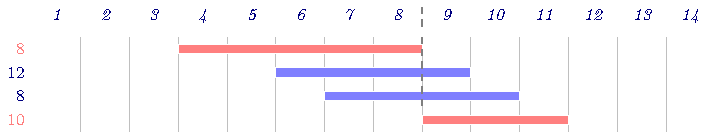
\includegraphics{assets/figures/13/gantt_part}
% 	\caption{Predecessore}%
% 	\label{fig:pred}
% \end{figure}
%
% \begin{figure}[H]
% 	\[
% 	DP[i] =
% 	\begin{dcases}
% 		0 & i = 0 \\
% 		\max (DP[i-1],\ \mathcolor{mathcolor}{DP[\mathit{pred}_i] + w_i)} & i > 0
% 	\end{dcases}
% 	\]
% 	\caption[pre-elaborazione intervalli pesati seconda versione]{Seconda versione}
% 	\label{}
% \end{figure}
%
% L'algoritmo di calcolo dei predecessori è illustrato di seguito
%
% \begin{algorithm}[H]
% 	\caption{}
% 	%&../preamble

% arara: pdflatex: { synctex: no }
% arara: latexmk: { clean: partial }
\ifstandalone
\begin{document}
\begin{algorithm}[H]
\fi

\tcp{Pre-computa i predecessori}
\prototype{\Array{\Int} \computePredecessor{\Array{\Int} a, \Array{\Int} a, \Int n}}{

	\BlankLine
	\Matrix{\Int} \(pred\) \(\Assign\) \new \Array{\Int}{0}{n}\;
	\(pred[0] \Assign 0\)\;

	\BlankLine
	\From{\(i \Assign 1\) \DownTo \(n\)}{
		\(j \Assign i-1\)\;

		\BlankLine
		\While{\(j > 0\) \And \(b[j] > a[i]\)}{
			\(\Decrement{j}\)\;
		}
		\(pred[i] \Assign j\)\;
	}

	\BlankLine
	\Return \(pred\)\;
}

\ifstandalone
\end{algorithm}
\end{document}
\fi

% \end{algorithm}
%
% \paragraph{Complessità}
% Pre-calcolare i predecessori viene a costare \(\Omicron(n^2)\), ma si può fare meglio di così.
%
% \begin{algorithm}[H]
% 	\caption{}
% 	%&../preamble

% arara: pdflatex: { synctex: no }
% arara: latexmk: { clean: partial }
\ifstandalone
\begin{document}
\begin{algorithm}[H]
\fi

\prototype{\Set \maxInterval{\Int a, \Int b, \Int w, \Int n}}{

	\{ ordina gli intervalli per estremi di fine crescenti \}\;

	\BlankLine
	\Matrix{\Int} \(pred\) \Assign \computePredecessor{a, b, n}\;
	\Matrix{\Int} \(DP\) \Assign \new \Array{\Int}{0}{n}\;

	\BlankLine
	\tcp{Riempio la tabella}
	\(DP[0] \Assign 0\)\;

	\BlankLine
	\tcp{Calcolo delle soluzioni}
	\From{\(i \Assign 1\) \DownTo \(n\)}{
		\(DP[i]\) \Assign \MathMax{\(DP[i-1]\), \(w[i] + DP[pred[i]]\)}\;
	}

	\tcp{Costruisco l'insieme dei predecessori}
	\(i \Assign n\)\;
	\Set \(S \Assign \setConstructor\)\;

	\BlankLine
	\While(\Comment*[h]{fintanto che ci sono intervalli disponibili}){\( i > 0 \)}{

		\BlankLine
		\eIf(\Comment*[h]{logica dell'algoritmo}){\(DP[i-1] > \weight{i} + DP[pred[i]]\)}{
			\(\Decrement{i}\) \Comment*[h]{non considerare l'intervallo}\;
		}{
			\(S.\setInsert(i)\) \Comment*[h]{inseriscilo nell'insieme}\;
			\(i \Assign pred[i]\) \Comment*[h]{scorri gli interalli}\;
		}
	}

	\BlankLine
	\Return \(S\) \Comment*[h]{ritorna l'insieme di intervalli ordinati}\;
}

\ifstandalone
\end{algorithm}
\end{document}
\fi

% \end{algorithm}
%
% \paragraph{Complessità}
% La complessità di questa funzione è la sommatoria asintotica di tutte le sue parti
%
% \begin{table}[H]
% 	\centering
% 	\begin{tabular}{@{} ll @{}}\toprule
% 		Funzione						& Costo						\\\midrule
% 		Ordinamento intervalli			& \(\Omicron(n \log n)\)	\\\lightrule
% 		Calcolo predecessori			& \(\Omicron(n \log n)\)	\\\lightrule
% 		Riempimento tabella \emph{DP} 	& \(\Omicron(n)\) 			\\\lightrule
% 		Ricostruzione soluzione			& \(\Omicron(n)\)			\\\cmidrule{2-2}
% 										& \(\Omicron(n \log n)\)	\\\bottomrule
% 	\end{tabular}
% \end{table}
%
% \begin{note}
% Talvolta, può essere necessario pre-processare l'input per poter applicare nella maniera più efficiente possibile la programmazione dinamica.
% \end{note}
%
% \section{Conclusioni}
%
% La programmazione dinamica non è la soluzione di tutti i vostri problemi.
% Esistono altre tecniche che possono fare \emph{meglio di così}.
% Inoltre, è possibile che soluzioni ad-hoc possano essere migliori.

\ifsubfile
\end{document}
\fi
